\chapter{実車走行の結果}
\label{chap:field}
本章では，2026年10月12日と10月27日に実施した実車走行の結果を述べる．10月12日は車両応答の同定と上限速度4\,m/sで3周する走行，10月27日は3〜5.5\,m/sでの周回走行を行った．

\section{走行条件}
\label{sec:field_cond}
走行はAI-Formulaのコースで行った．1周の長さは，走行軌跡のGNSS経路長で赤コース約261\,m，青コース約257\,m（車輪速度の積算では約256\,m，253\,m）であり，車線幅の設定値（局所経路計画）は4\,mである（地図上の車線幅は約3.65\,m，Fig.~\ref{fig:run55_ts}の凡例）．10月12日は赤コースを4\,m/sで走行する自律走行を1本（2周と3周目の途中まで）と，手動操縦による同定走行を6本（4〜7\,m/s）行った．10月27日は，赤コースと青コースで上限速度3〜5.5\,m/sの自律走行を計17本行った．経路追従制御は，10月12日はMPC，10月27日は序盤の2本がPure Pursuit法，以降はMPCである．経路生成の重みは，記録した画像を候補の重みで再推論し記録された経路と照合して特定した．10月12日は9月27日版（RMSE 2.5\,mm），10月27日は10月24日版（R2の30フレームでRMSE 15.7\,mm，中央値7.1\,mm，他の候補は350\,mm以上）である．信号パネルは10月12日は消灯で走行し，10月27日は点灯したパネルで走行した（R2の記録画像で赤の点灯を確認し，検出結果に赤443件・緑101件の両方がある）．

Table~\ref{tab:config}に，各走行で動作したソフトウェアの構成を示す．2章に示した本システムは最終構成であり，10月12日の走行は3次多項式の平滑化，停止減速度の分離，回避側の保持，分岐での速度抑制，トポロジカルマップによる経路選択の導入前である．10月27日は車両側の計算機で変更を加えた版で走行しており，その版は版管理に取り込まれていないため，構成は変更の履歴と記録から特定した．平滑化の次数は，記録された平滑化後の経路に1〜4次の多項式を当てはめた残差から判定した（200フレームの中央値で，10月27日の3本は2次で92〜274\,mm，3次で$10^{-4}$\,mm以下，10月12日は2次で$10^{-4}$\,mm以下）．分岐での速度抑制は，B1の記録で経路選択の指示が直進以外のあいだ速度計画の上限が4.0\,m/sに下がっていることから確認した（\ref{sec:decomp_result}節）．

\begin{table}[H]
  \centering
  \caption{Software configuration of each run.}
  \label{tab:config}
  \scriptsize
  \begin{tabular}{L{2.4cm}L{2.2cm}L{2.2cm}L{2.2cm}L{2.2cm}}
    \toprule
    項目 & 10/12 & 10/27 R1, R2 & 10/27 B1〜B9 & 10/27 R3〜R8 \\
    \midrule
    版 & b68bfd1（版管理に未登録の変更あり） & 車両側で変更（版管理に未登録） & 同左 & 同左 \\
    経路追従制御 & MPC & Pure Pursuit法 & MPC & MPC \\
    速度計画の$a_{x,\max}$ [m/s$^2$] & 6.0 & 3.0 & 3.0 & 3.0 \\
    経路の平滑化 & 2次，12\,m & 3次，12\,m & 同左 & 同左 \\
    合流距離 & 固定15\,m & 速度比例，4〜15\,m & 同左 & 同左 \\
    停止減速度の分離 & なし & あり & あり & あり \\
    回避側の保持 & なし & あり & あり & あり \\
    分岐での速度抑制 & なし & なし & あり（上限4.0\,m/s） & なし \\
    経路選択の指示 & 常に直進 & 常に直進 & トポロジカルマップ & 常に直進 \\
    経路生成の重み & 9月27日版 & 10月24日版 & 10月24日版 & 10月24日版 \\
    上限速度 [m/s] & 4.0 & 3.0, 4.0 & 4.5, 5.0, 5.3 & 5.5, 5.0, 4.0 \\
    信号パネル & 消灯 & 点灯 & -- & 点灯 \\
    \bottomrule
  \end{tabular}
\end{table}

Table~\ref{tab:runs}に10月27日の走行の一覧を示す．速度は自律走行中の実測並進速度の中央値，表中の「3.5\,m/s超」は並進速度が3.5\,m/sを超えていた区間の走行時間の合計，横偏差は経路生成が推定した車線中心（平滑化後の参照経路）に対する自車位置の横偏差の絶対値の95パーセント点，舵角の変化率は舵角の指令値の絶対変化率の平均，IMU欠落率は慣性航法装置の出力が0.2\,s以上途絶えていた時間の割合である．横偏差の基準は経路生成の出力であり，コースに対する独立な基準ではないことに注意する．R3は車輪速度が大部分で記録されていないため，速度（5.5）は上限速度の設定値，横偏差（1.5）は概略値であり，他の走行と同じ算出ではない．走行の記号は赤コースをR，青コースをBとし，表は時系列順である．Fig.~\ref{fig:run1027_summary}に，各走行の速度に対する横偏差とIMU欠落率を示す．表中の完走の定義は\ref{sec:field_method}節に示す．

\begin{table}[H]
  \centering
  \caption{Autonomous driving runs on October 27, 2026.}
  \label{tab:runs}
  \scriptsize
  \begin{tabular}{llrrrrrL{2.4cm}}
    \toprule
    走行 & コース & 速度 [m/s] & 3.5\,m/s超 [s] & 横偏差 [m] & 舵角 [$^\circ$/s] & IMU欠落 [\%] & 結果 \\
    \midrule
    R1 & 赤 & 3.0 & 12 & 1.62 & 5 & 0 & Pure Pursuit，短時間（速度条件なしで集計） \\
    R2 & 赤 & 3.9 & 187 & 0.23 & 5 & 0 & 完走（3周，信号停止あり） \\
    B1 & 青 & 4.4 & 168 & 0.33 & 8 & 0 & 2.97周（上限4.5\,m/s，3周目の97\%で介入） \\
    B2 & 青 & 4.9 & 130 & 1.20 & 8 & 1 & 分岐で失敗 \\
    B3 & 青 & 4.9 & 32 & 1.32 & 9 & 0 & 分岐で失敗 \\
    B4 & 青 & 4.8 & 31 & 1.24 & 12 & 8 & 分岐で失敗 \\
    B5 & 青 & 4.9 & 161 & 0.78 & 9 & 3 & 2周目の分岐で失敗 \\
    B6 & 青 & 4.9 & 55 & 0.85 & 7 & 0 & 分岐で失敗 \\
    B7 & 青 & 4.9 & 30 & 0.81 & 9 & 3 & 分岐で失敗 \\
    B8 & 青 & 4.9 & 27 & 0.34 & 13 & 27 & 分岐で失敗 \\
    B9 & 青 & 5.3 & 106 & 0.97 & 2 & 13 & 途中で介入 \\
    R3 & 赤 & 5.5 & 70 & 1.5 & -- & -- & 隣接車線へ移動 \\
    R4 & 赤 & 4.8 & 41 & 0.97 & 38 & 66 & 蛇行，介入 \\
    R5 & 赤 & 4.8 & 33 & 0.87 & 33 & 38 & 蛇行，介入 \\
    R6 & 赤 & 4.9 & 24 & 0.33 & 12 & 83 & 短時間 \\
    R7 & 赤 & 4.8 & 136 & 1.32 & 18 & 54 & 蛇行，介入 \\
    R8 & 赤 & 3.9 & 156 & 0.79 & 5 & 0 & 完走（3.6周，信号停止3回，走行後に車両側が停止） \\
    \bottomrule
  \end{tabular}
\end{table}

\begin{figure}[H]
  \centering
  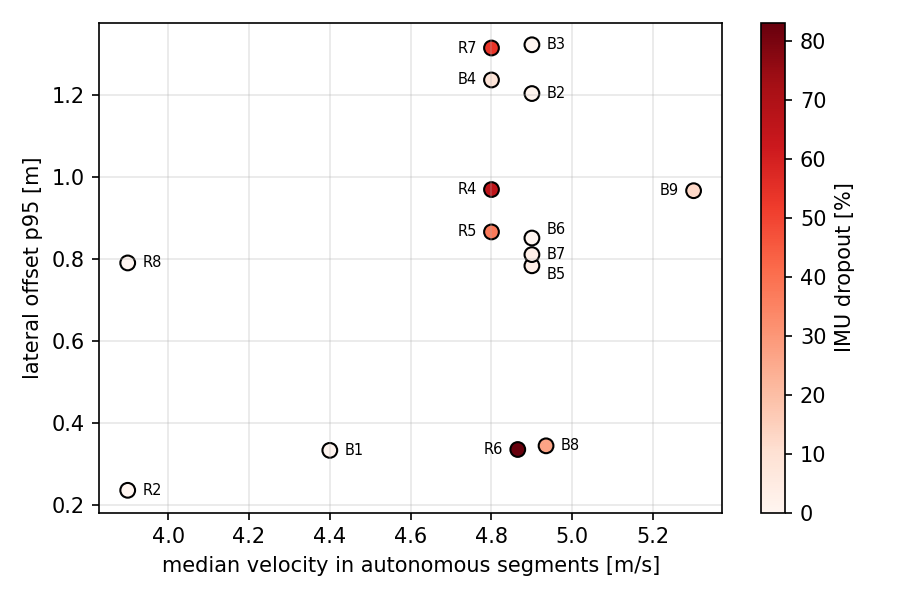
\includegraphics[width=0.6\textwidth]{images/run1027_summary.png}
  \caption{Lateral offset (95th percentile) versus median velocity for the runs on October 27. The color shows the IMU dropout ratio. Each point is labeled with its run symbol (R2, B1--B9, R4--R8); B8 and R6 are shifted by $\pm 0.035$\,m/s in $x$ to avoid overlap. The 15 points do not include R1 (a short run at 3.0\,m/s) and R3 (the wheel speed was not recorded for most of the run).}
  \label{fig:run1027_summary}
\end{figure}

\section{車両応答の同定結果}
\label{sec:ident_result}
10月12日の手動走行から同定した車両応答をTable~\ref{tab:ident}に示す．Fig.~\ref{fig:ident_speed}に並進速度の指令値に対する応答を，Fig.~\ref{fig:ident_steer}に舵角の指令値に対する応答の同定値を示す．並進速度は，むだ時間0.20〜0.27\,sと一次遅れ0.39〜0.65\,sで表され，加速の上限は3.4\,m/s$^2$，減速の上限は3.6\,m/s$^2$であった（決定係数0.98）．舵角の指令値に対する等価舵角の応答は，3\,m/s以上でゲイン約1.0，時定数0.10〜0.17\,s，むだ時間0.03〜0.11\,sであり，両者の合計は0.15〜0.24\,s（3，4，5，6\,m/sでそれぞれ0.15，0.24，0.20，0.21\,s）であった．従動輪の実舵角と等価舵角の時間差は10〜20\,msでほぼ同期しており，傾きは1.05〜1.24であった．これは公称のホイールベース0.733\,mに対して0.59〜0.70\,mの有効ホイールベースに相当する（約5〜20\%短い）．認識から制御までの遅延は平均0.106\,s（95パーセント点0.15\,s）であった．

また，Fig.~\ref{fig:ident_shimmy}に示すように，従動輪には約8\,Hzのシミーが4\,m/sから現れ，直進でも自励的に成長した（成長率の中央値4.2\,s$^{-1}$）．6.5\,m/sでは発散して横滑りに至ったため，本研究では6\,m/sを超える走行は行わない．

10月27日の自律走行中の舵角の指令値と従動輪の実舵角から，同じ一次遅れとむだ時間のモデルを走行ごとに当てはめたところ（15本），ゲインは1.17$\pm$0.31（0.69〜1.64），時定数は0.44$\pm$0.14\,s（推定値が探索範囲の上限に達した1本を除く），むだ時間は0〜0.30\,sであった．手動の段階入力による同定値に比べてばらつきが大きく，時定数は約3倍である．自律走行中の指令は励起が小さいこと，走行ごとに速度と路面が異なることから，速度計画と閉ループシミュレーションの車両モデルには手動走行による同定値を用いるが，自律走行中の当てはめ値が実際の走行条件に近い可能性は否定できず，\ref{sec:limitations}節で限界として述べる．

\begin{table}[H]
  \centering
  \caption{Identified vehicle response.}
  \label{tab:ident}
  \begin{tabular}{lll}
    \toprule
    項目 & 同定値 & 備考 \\
    \midrule
    並進速度のむだ時間 & 0.20〜0.27\,s & \\
    並進速度の一次遅れ & 0.39〜0.65\,s & 定常偏差 $-2$\%（4\,m/s），$-9$\%（6\,m/s） \\
    加速の上限 & 3.4\,m/s$^2$ & \\
    減速の上限 & 3.6\,m/s$^2$ & 実測最大 3.7〜4.4\,m/s$^2$ \\
    舵角応答のゲイン & 約1.0 & 3\,m/s以上 \\
    舵角応答の遅れ & 0.15〜0.24\,s & むだ時間と一次遅れの合計 \\
    有効ホイールベース & 0.59〜0.70\,m & 公称0.733\,m，傾き1.05〜1.24に対応 \\
    認識から制御までの遅延 & 0.106\,s & 95パーセント点 0.15\,s \\
    \bottomrule
  \end{tabular}
\end{table}

\begin{figure}[H]
  \centering
  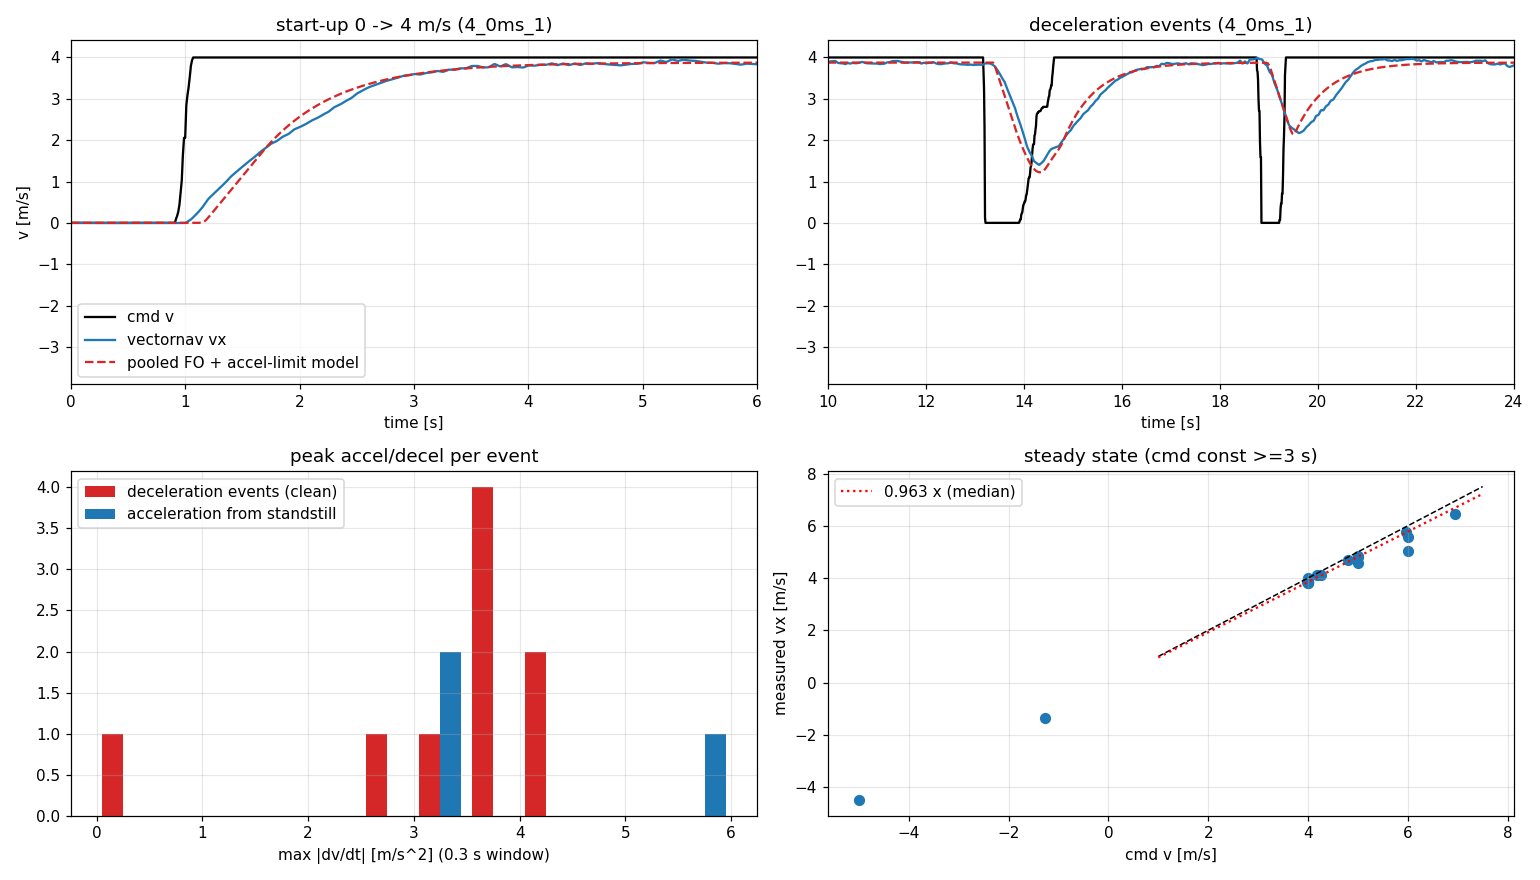
\includegraphics[width=0.85\textwidth]{images/ident_speed_response.png}
  \caption{Response of the measured velocity to the velocity command (manual driving on October 12).}
  \label{fig:ident_speed}
\end{figure}

\begin{figure}[H]
  \centering
  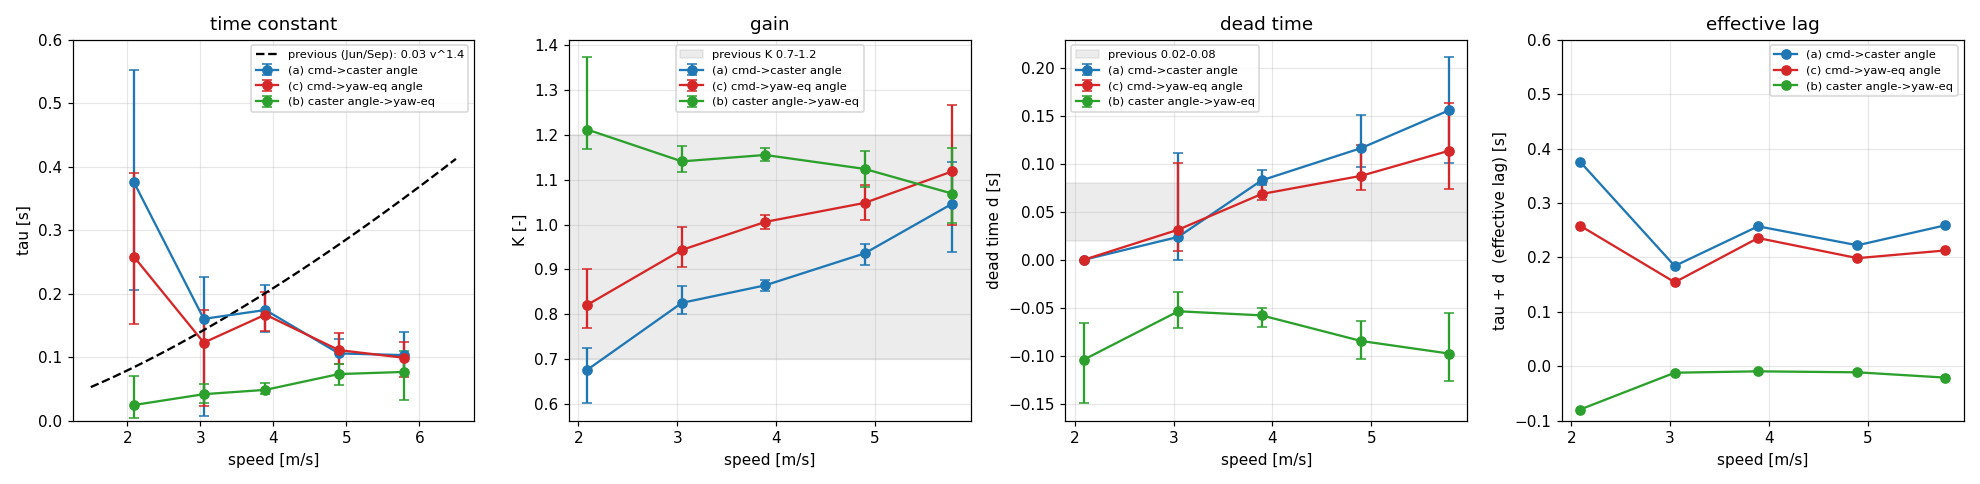
\includegraphics[width=0.95\textwidth]{images/ident_steer_response.png}
  \caption{Identified time constant, gain, dead time, and effective lag of the steering response versus velocity.}
  \label{fig:ident_steer}
\end{figure}

\begin{figure}[H]
  \centering
  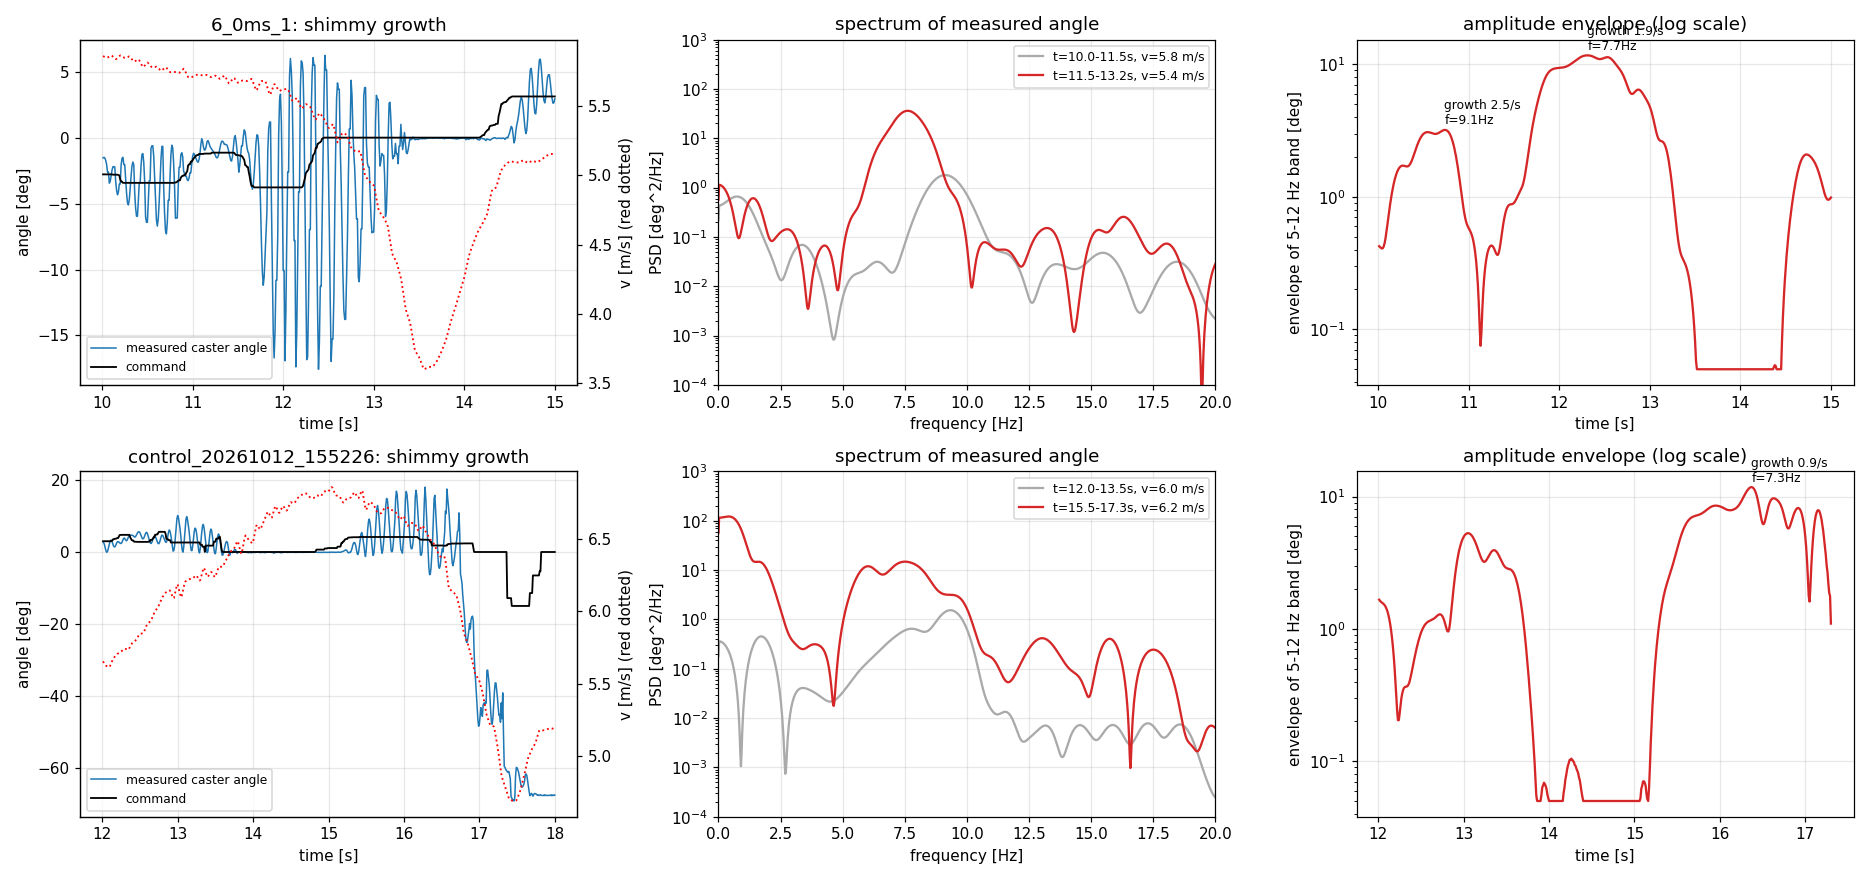
\includegraphics[width=0.95\textwidth]{images/ident_shimmy.png}
  \caption{Shimmy of the caster: time series of the caster angle, its spectrum, and the amplitude envelope in the run at 6\,m/s (top) and in the run in which the shimmy diverged at 6.5\,m/s (bottom).}
  \label{fig:ident_shimmy}
\end{figure}

\section{4\,m/sでの周回走行}
\label{sec:run4}
上限速度4\,m/s（B1は4.5\,m/s）では，赤コースの10月27日のR2とR8は介入なしで3周を走行して完走し（\ref{sec:field_method}節の定義），青コースの10月27日のB1は2.97周を走行したが，3周目の基準線の約7\,m手前で手動により制動したため完走には含めず，3周目は周長の97\%までを解析に用いる．10月12日の赤コースは2周を走行し，3周目の途中（基準線の約110\,m手前）で自律走行を終えた．R8は信号停止を3回行い（停止保持5.4，4.8，15.1\,s．3回目は停止後に動き出して停止線を越え，再停止を2回繰り返した），3周の基準線通過ののちも走行を続け（走行距離は3.6周分），その後車両側の通信が停止して走行を終えた（解析は3周目の基準線通過までである）．Table~\ref{tab:laptimes}に，各走行のラップタイムを示す．ラップタイムは，自律走行の開始点を通り進行方向に直交する基準線をGNSSの軌跡が通過した時刻の差とした．Fig.~\ref{fig:run1012_traj}に10月12日の走行軌跡を，Fig.~\ref{fig:run1012_track}に経路追従誤差の時系列を示す．10月12日の赤コース2周の平均速度は，GNSSの経路長（261.0\,m，264.7\,m）とラップタイムの合計137.0\,sからは3.84\,m/sであり，Table~\ref{tab:decomp}の走行距離と時間（2.57周，663.9\,m，184.6\,s，停止3回と3周目の部分周を含む）からは3.60\,m/sである．

\begin{table}[H]
  \centering
  \caption{Measured lap times of the runs at a 4\,m/s limit (crossing of the start line by the GNSS trajectory).}
  \label{tab:laptimes}
  \small
  \begin{tabular}{llrrrL{4.2cm}}
    \toprule
    走行 & コース（上限速度） & 1周目 [s] & 2周目 [s] & 3周目 [s] & 備考 \\
    \midrule
    10/12 & 赤（4.0\,m/s） & 68.52 & 68.51 & -- & 3周目は途中で終了，停止3回 \\
    R2 & 赤（4.0\,m/s） & 72.30 & 77.31 & 69.38 & 信号停止3回 \\
    B1 & 青（4.5\,m/s） & 60.54 & 59.75 & (60.86) & 3周目は制動中に通過 \\
    R8 & 赤（4.0\,m/s） & 74.47 & 78.94 & 96.23 & 信号停止3回，3周目に再停止 \\
    \bottomrule
  \end{tabular}
\end{table}

10月12日の経路追従誤差は，局所経路に対する横偏差のRMSが0.056\,m（95パーセント点0.093\,m），平滑化後の目標経路に対しては0.27\,m（95パーセント点0.57\,m）であった．局所経路は毎周期，計測した自己位置から再計算されるため，局所経路に対する誤差は小さく評価される．Fig.~\ref{fig:run4_ts}に10月27日のR2とB1の速度，横偏差，舵角の指令値の時系列を，Fig.~\ref{fig:run1027_topdown}にB1の走行軌跡を示す．青コースのB1は，トポロジカルマップから生成した経路選択の指示で交差点を3周通過した．経路生成が推定した車線中心に対する横偏差の95パーセント点は，R2で0.23\,m，B1で0.33\,m，R8で0.79\,mであった．R8の値が大きいのは，3周目に経路の曲率の雑音による減速と蛇行が生じたためである．Fig.~\ref{fig:rviz_blue}に走行中の可視化画面を示す．

\begin{figure}[H]
  \centering
  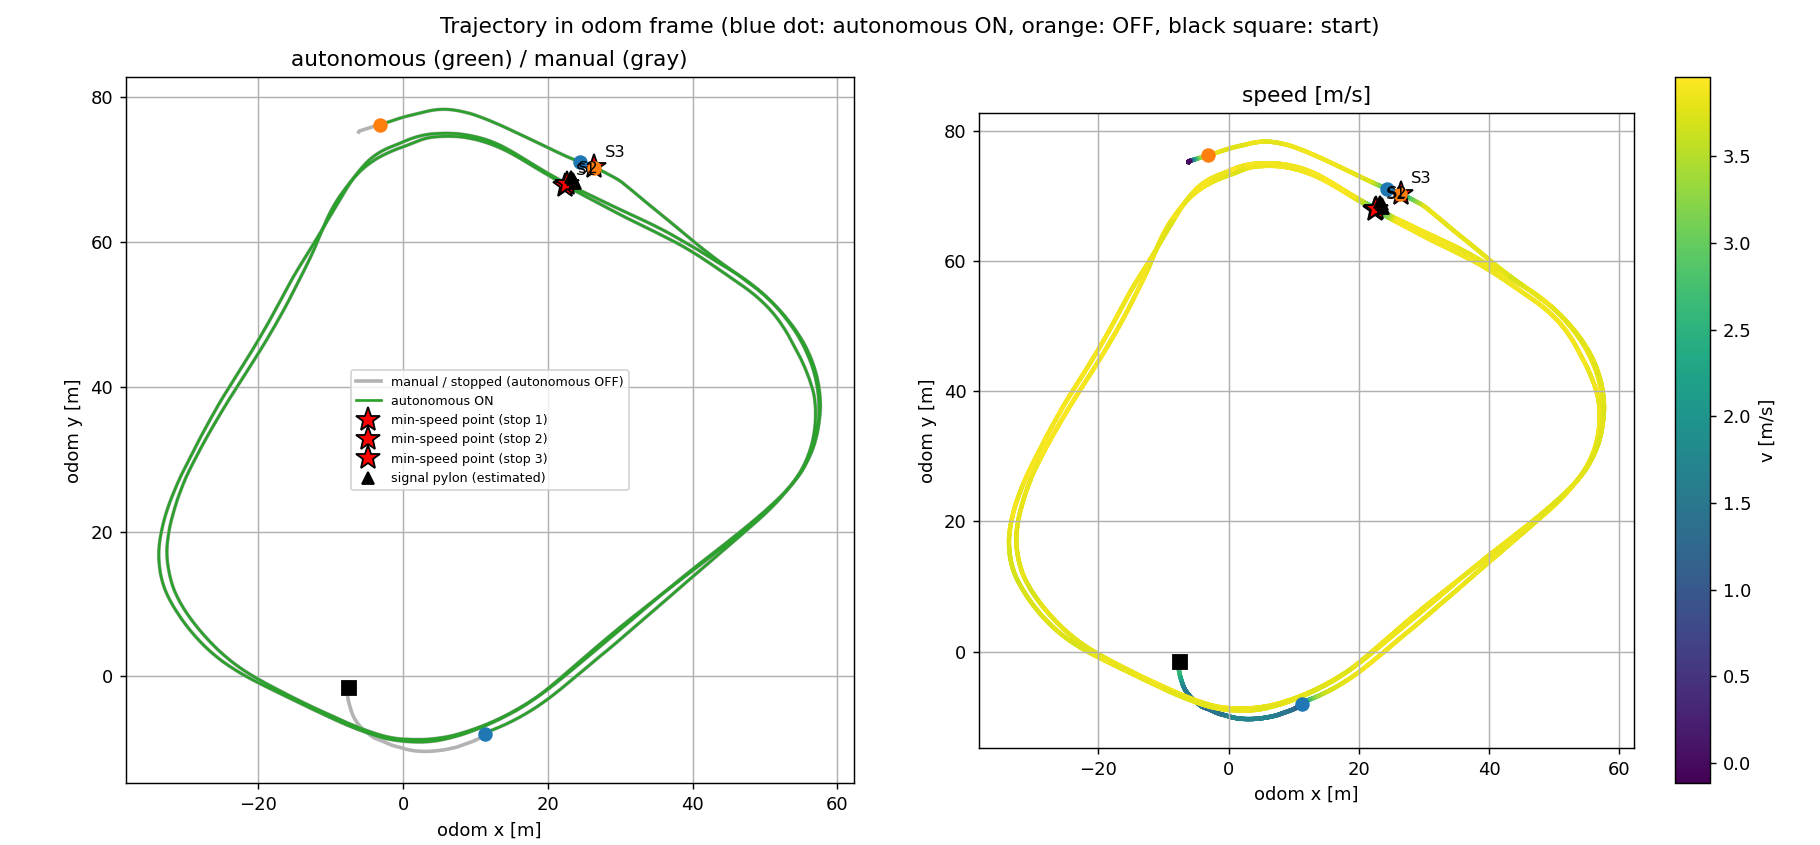
\includegraphics[width=0.95\textwidth]{images/run1012_trajectory.png}
  \caption{Trajectory of the run on the red course at a 4\,m/s limit (October 12, 2.57 laps). Left: autonomous (green) and manual (gray) segments. Right: velocity.}
  \label{fig:run1012_traj}
\end{figure}

\begin{figure}[H]
  \centering
  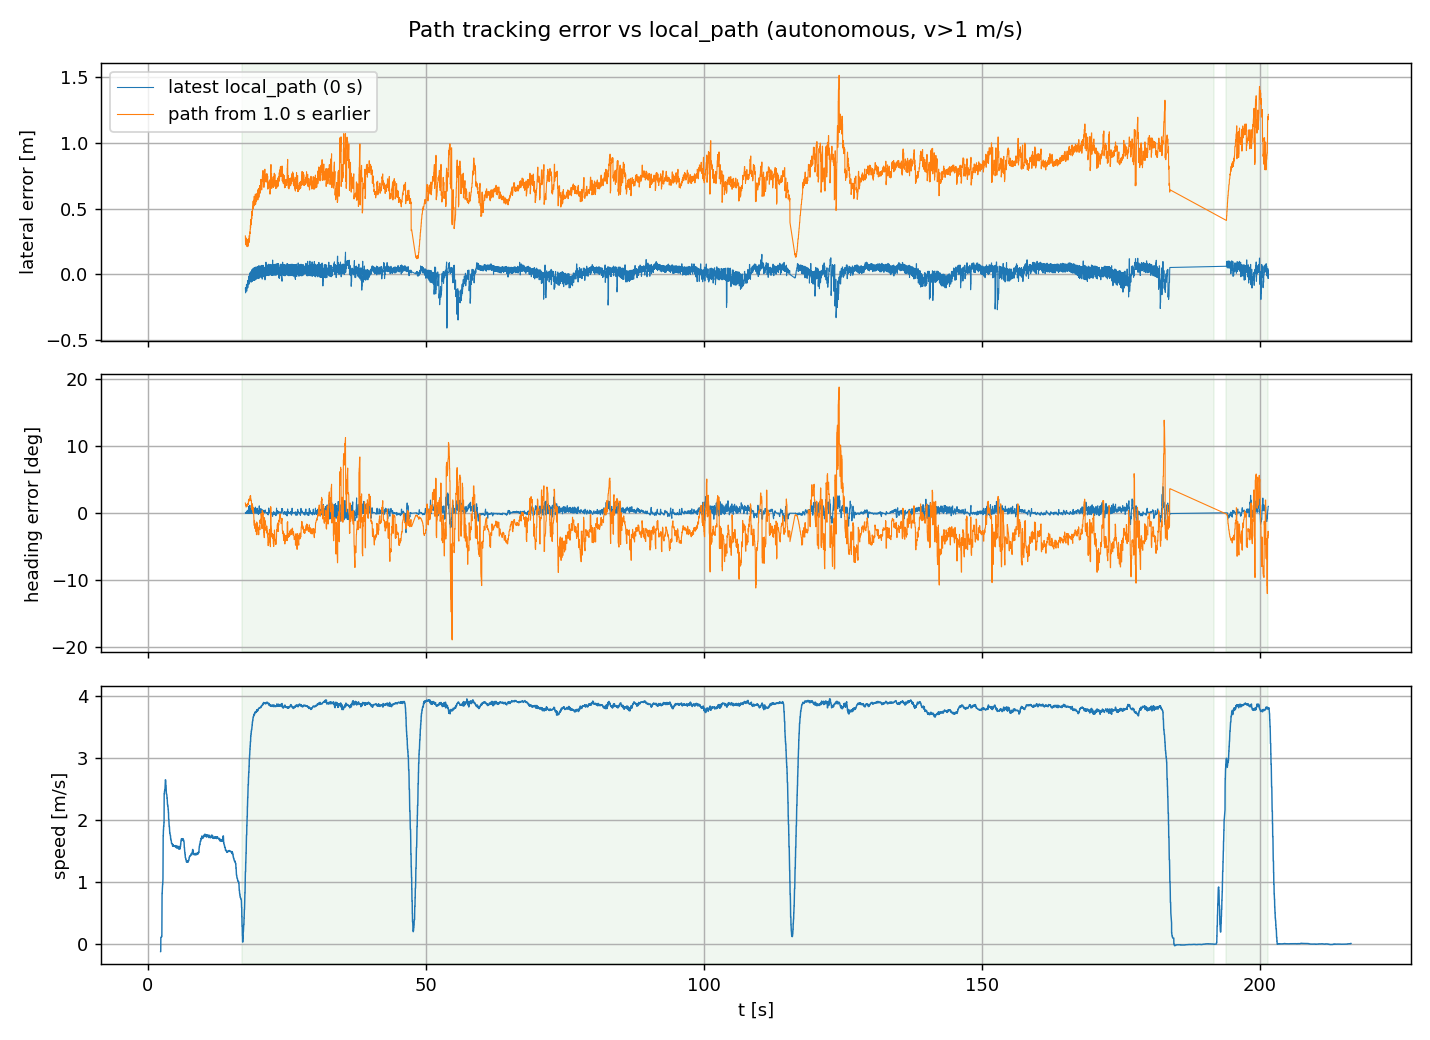
\includegraphics[width=0.95\textwidth]{images/run1012_tracking_error.png}
  \caption{Path-following error with respect to the local path (October 12, 4\,m/s): lateral error, heading error, and velocity.}
  \label{fig:run1012_track}
\end{figure}

\begin{figure}[H]
  \centering
  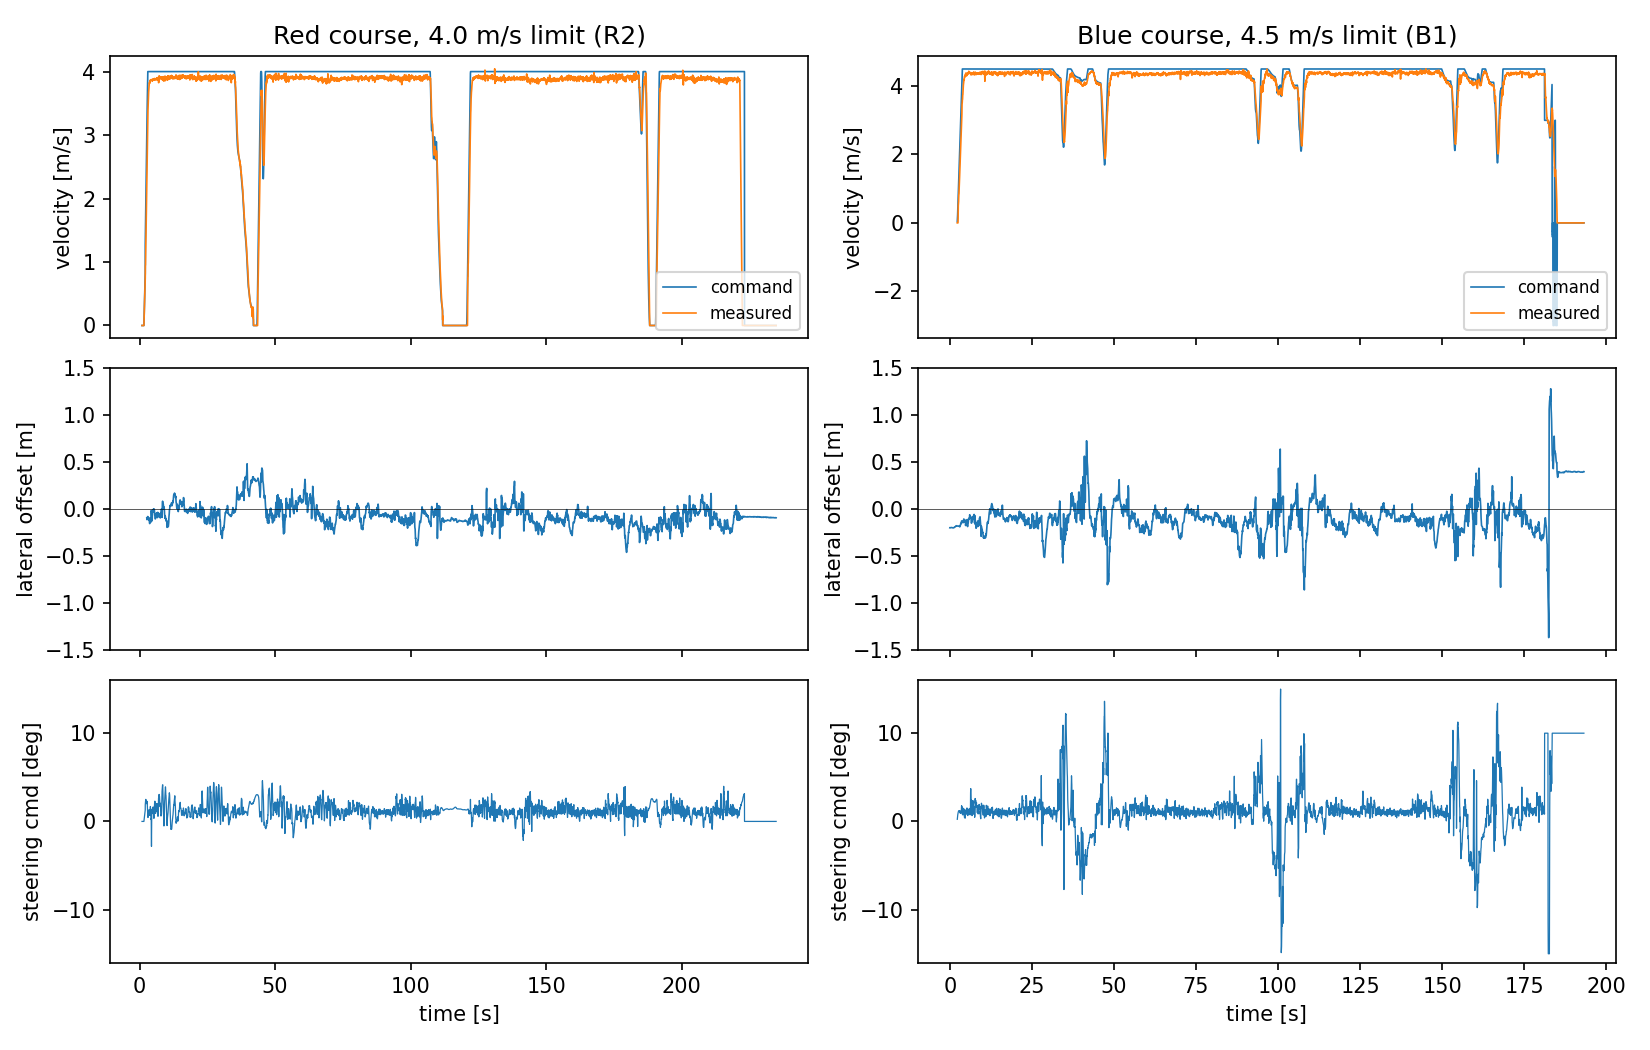
\includegraphics[width=0.98\textwidth]{images/run4_timeseries.png}
  \caption{Time series of velocity, lateral offset from the estimated lane center, and steering command on October 27 (left: R2, red course, 4.0\,m/s limit; right: B1, blue course, 4.5\,m/s limit).}
  \label{fig:run4_ts}
\end{figure}

\begin{figure}[H]
  \centering
  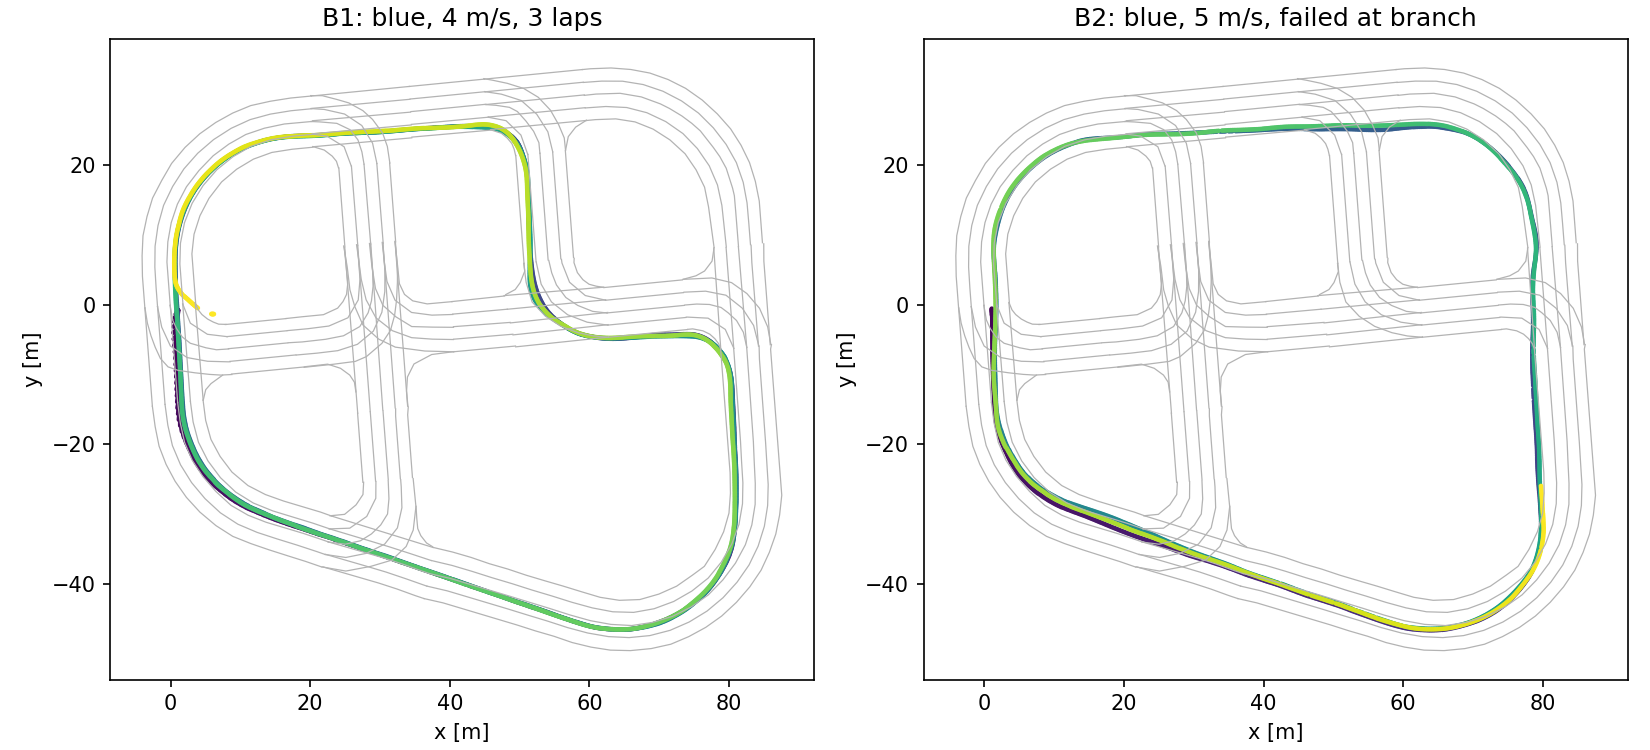
\includegraphics[width=0.98\textwidth]{images/run1027_topdown.png}
  \caption{GNSS trajectories of the autonomous segments over the lane lines (left: B1, blue course, 4.5\,m/s limit; right: B2, blue course, 5\,m/s limit). The color shows the elapsed time.}
  \label{fig:run1027_topdown}
\end{figure}

\begin{figure}[H]
  \centering
  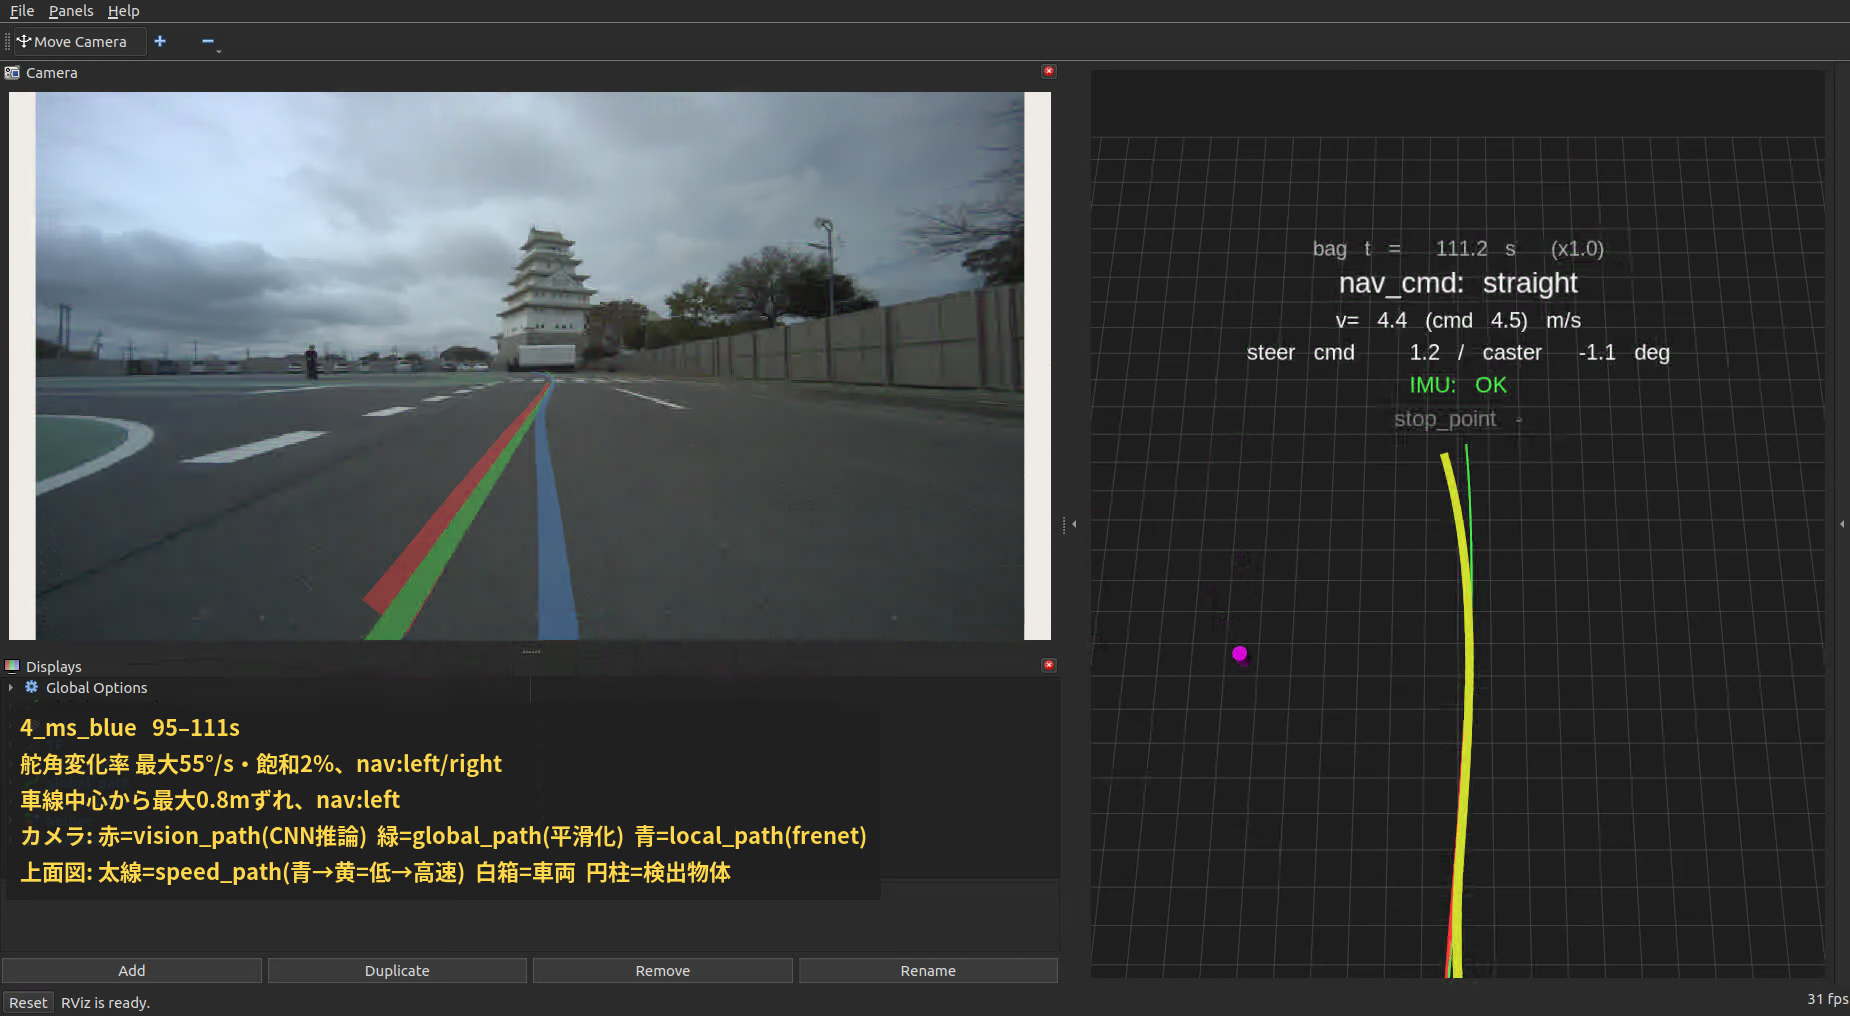
\includegraphics[width=0.9\textwidth]{images/rviz_blue_4ms.png}
  \caption{Visualization during the blue-course run B1 (4.5\,m/s limit): camera image, generated path, and local path.}
  \label{fig:rviz_blue}
\end{figure}

経路生成の出力は，Fig.~\ref{fig:run1012_stability}に示すように，フレーム間で前方3，5，8\,mにおいて横位置がRMSで0.13，0.19，0.35\,m揺らぎ，平滑化後も0.11，0.17，0.31\,mであった．平滑化の時間窓0.15\,sは15\,Hzでは2〜3フレーム分にすぎず，時間方向の平滑化としてはほとんど働いていない．舵角の指令値には1\,Hzを超える成分がRMSで0.96$^\circ$含まれ，その約半分は経路の更新に伴う段差に起因した．

\begin{figure}[H]
  \centering
  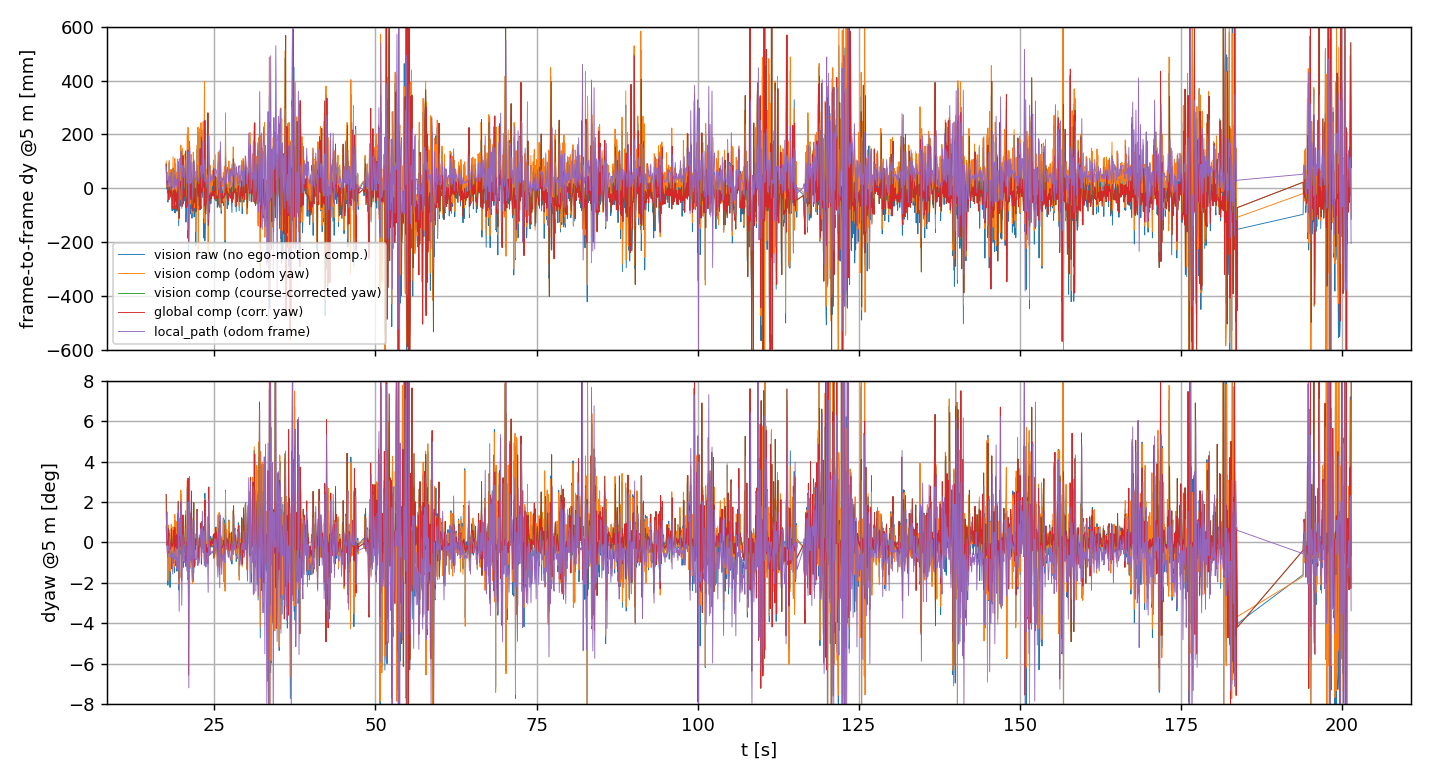
\includegraphics[width=0.95\textwidth]{images/run1012_path_stability.png}
  \caption{Frame-to-frame fluctuation of the generated path at 5\,m ahead (October 12): lateral position (top) and heading (bottom).}
  \label{fig:run1012_stability}
\end{figure}

10月12日は信号パネルが消灯しており，消灯したパネルを赤と誤って判定したことによる停止が3回生じた．この停止は信号停止と同じ処理で生じるため，停止の挙動の解析に用いる．3回目の停止では，赤と判定してから停止するまでに停止点を0.81\,m行き過ぎた．停止点が最初に発行されたときの認識上の停止点までの距離は，10月12日で約5.3\,m，点灯したパネルで走行した10月27日のR2で6.98\,mであった（真の距離は\ref{sec:stop_result}項で見積もる）．Fig.~\ref{fig:run1012_stop}に示すように，同定値の範囲内の車両モデル（むだ時間0.27\,s，一次遅れ0.39\,s）で閉ループ再現したところ行き過ぎは0.73\,mであった．再現モデル上で要因を1つずつ取り除いたときの行き過ぎの変化は，車両のむだ時間と一次遅れで1.9\,m，検出と計画の遅延で0.6\,m，縦方向の制御（減速度の最小値とジャーク制限）で0.7\,m，減速能力の差で0.3\,mであり，速度計画の0.3\,s先の参照は行き過ぎを1.9\,m減らしていた．これらは1つずつ取り除いた感度であり加法的ではないが，車両の遅れが最も大きい要因であることを示している．

\begin{figure}[H]
  \centering
  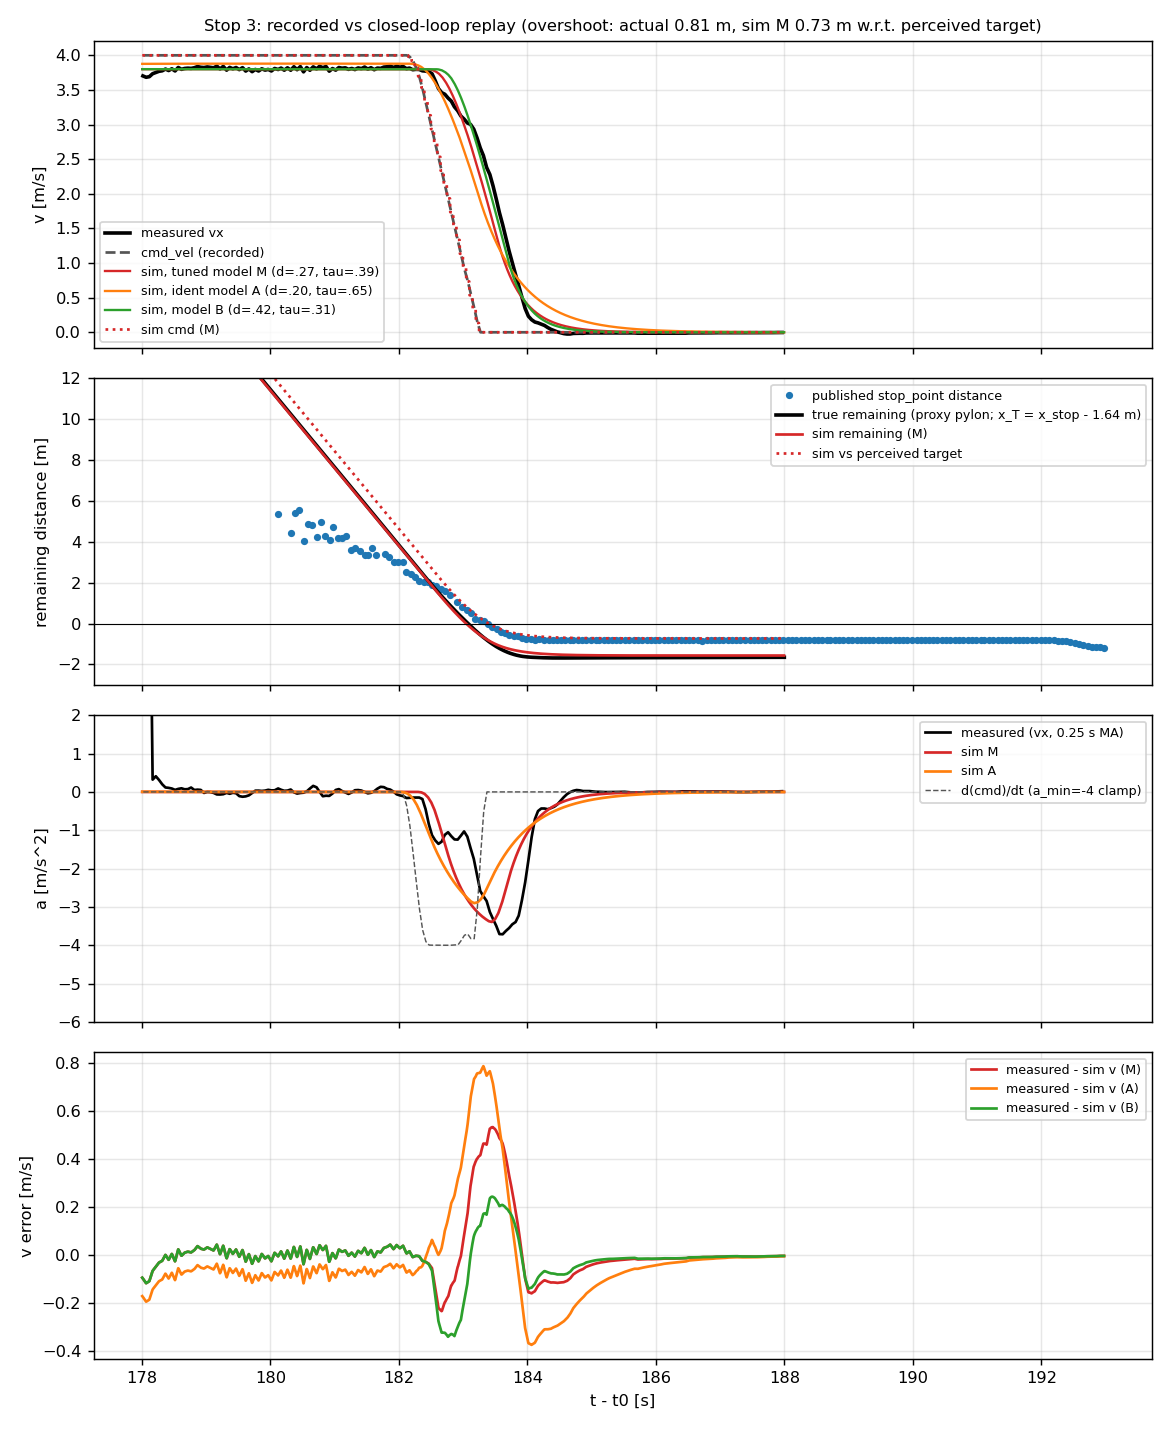
\includegraphics[width=0.7\textwidth]{images/run1012_stop_replay.png}
  \caption{Closed-loop reproduction of the signal stop (October 12, stop 3): velocity, remaining distance, acceleration, and velocity error.}
  \label{fig:run1012_stop}
\end{figure}

\section{5\,m/s以上での走行と失敗の要因}
\label{sec:run5}
上限速度を5\,m/s以上とした13本（Table~\ref{tab:runs}のB2〜B9，R3〜R7）のうち，3周を完走した走行はなかった．横偏差の95パーセント点は0.33〜1.5\,mであり，上限速度4\,m/sの0.23〜0.79\,mと重なる範囲にある．このうちB2〜B4は交差点で予定と異なる経路に入った区間を含むため，速度の効果だけを表す値ではない．失敗の要因を，画像，各段の経路，自己位置，指令値，車体の応答の記録から走行ごとに切り分けた結果をTable~\ref{tab:causes}に示す．要因は，(a) ソフトウェアの不具合とセンサの故障，(b) 要素の設計の限界，(c) 車両の特性，に分類した．

\begin{table}[H]
  \centering
  \caption{Main cause of failure identified for each run at 5\,m/s or above.}
  \label{tab:causes}
  \small
  \begin{tabular}{llL{6.5cm}l}
    \toprule
    走行 & 分類 & 主因と根拠 & 自律走行 [s] \\
    \midrule
    B2 & (a) & 経路選択の初期化の不備（地図が$-99^\circ$回転，指示が出ず） & 130 \\
    B3 & 未特定 & 左折指示後に横偏差1.6\,m．記録からは主因を特定できず & 32 \\
    B4 & 未特定 & 左折指示後に横偏差1.3\,m．同上 & 31 \\
    B5 & (a) & 慣性航法装置の再起動によるジャイロバイアスと方位の変化（2周目の分岐） & 161 \\
    B6 & (a) & 経路選択の初期化の不備（地図が$-179^\circ$回転） & 55 \\
    B7 & (b) & 右折の指示が早く，経路生成が手前の白線を誤検出 & 30 \\
    B8 & (a) & 経路選択の初期化の不備（約$65^\circ$回転）とIMU欠落27\% & 27 \\
    B9 & 未特定 & 右折指示の直後に横偏差1.0\,m，IMU欠落13\%．主因を特定できず & 106 \\
    R3 & (c)主，(b)副 & 指令と逆向きのヨー運動と，再計画・回避判断との相互作用（\ref{sec:yaw}項） & 70 \\
    R4, R5, R7 & (a) & IMU欠落中（38〜66\%）の舵角振動と蛇行 & 41, 33, 136 \\
    R6 & (a) & IMU欠落83\%，短時間で打ち切り & 24 \\
    \bottomrule
  \end{tabular}
\end{table}

13本のうち，(a) が8本，(b) が1本，(c) が1本，主因を特定できなかったものが3本である．要素の設計の関与が特定できたのはB7とR3の2本にとどまる．主因を特定できなかったB3，B4，B9はいずれも分岐の指示後の逸脱であり，要素の設計の関与を排除できない．また，多くの走行は24〜55\,sで打ち切られているため，高速での急カーブや交差点で要素の設計が試された区間は限られている．以下に各要因を述べる．

\subsection{自己位置推定の入力欠落}
慣性航法装置の出力が0.2\,s以上途絶える事象が17本中10本で生じ，最長の途絶は約20\,sであった．自己位置の姿勢は慣性航法装置の姿勢から求めているため，欠落中は車両が旋回しても姿勢が更新されず，自己位置が実際の向きからずれる．Fig.~\ref{fig:run5_imu}にR4の例を示す．欠落中および復帰直後には舵角の指令値の変化量が2〜6倍に増え，赤コースのR4，R5，R7の蛇行はこの区間で生じた．Fig.~\ref{fig:run5_imu}では，振動は欠落の最中よりも欠落からの復帰直後に大きく，復帰時に姿勢の推定値が跳ぶことが引き金になっている可能性がある．欠落中，復帰直後，通常の区間に分けた集計は今後の課題である．欠落後に装置が再起動し，ジャイロのバイアスと絶対方位が変化した例もあった（B5）．欠落率はTable~\ref{tab:runs}の時系列で後半ほど高く，最後に4\,m/sで走行したR8では0\%であったため，欠落は速度ではなく走行の時刻（装置の温度や電源）に関係している可能性があるが，原因は特定できていない．

\begin{figure}[H]
  \centering
  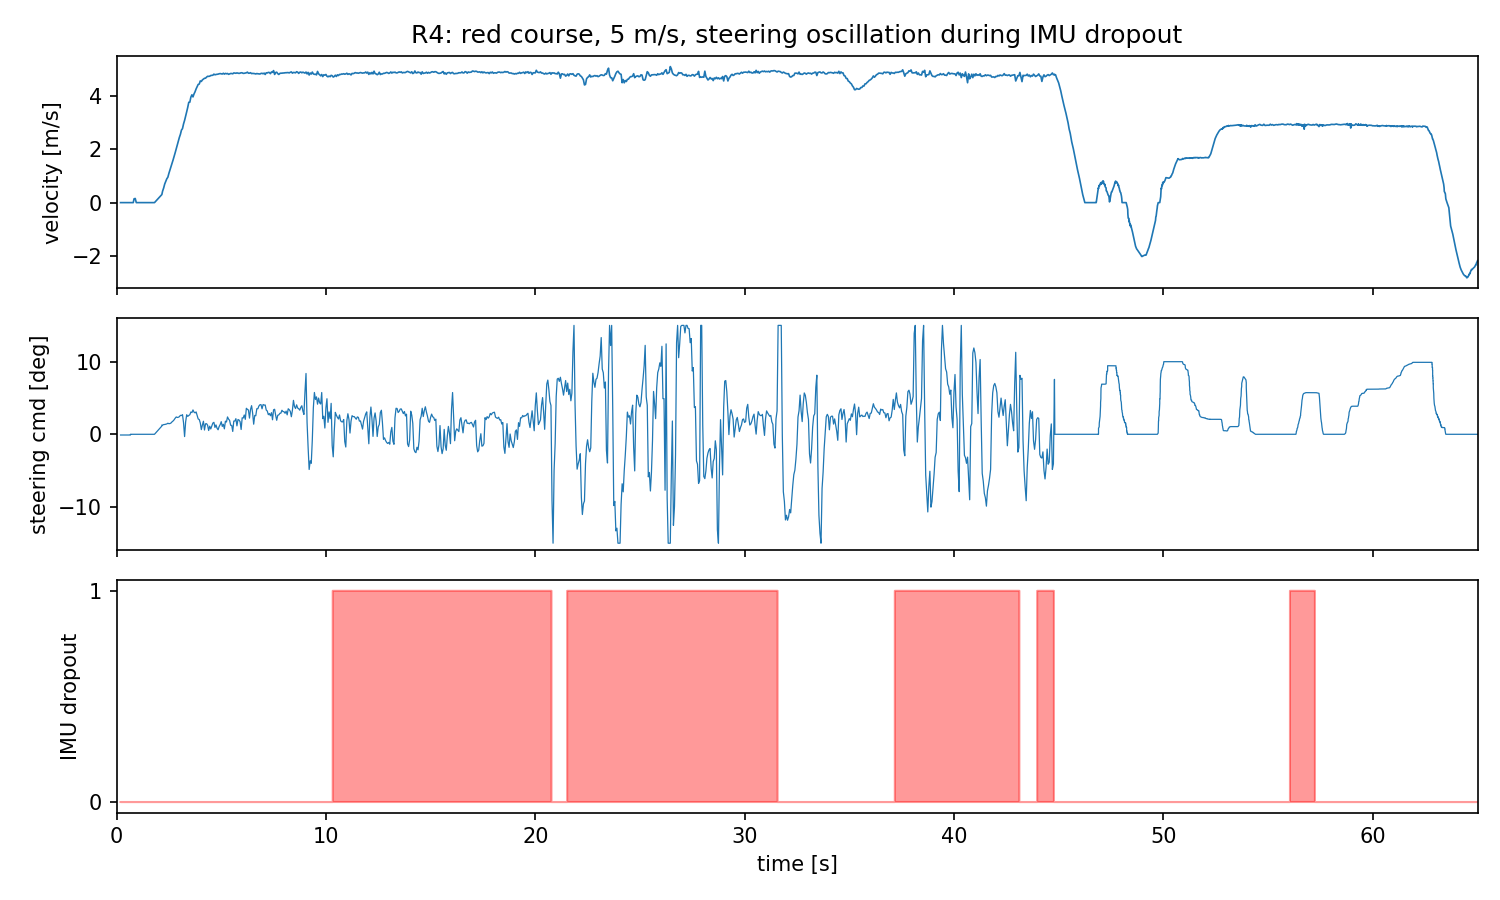
\includegraphics[width=0.95\textwidth]{images/run5_imu_dropout.png}
  \caption{Steering oscillation during IMU dropout (R4, red course at 5\,m/s): velocity, steering command, and dropout periods.}
  \label{fig:run5_imu}
\end{figure}

\subsection{経路選択の指示の初期化}
青コースでは，トポロジカルマップ上の位置を初期化する際に自己位置推定の姿勢を考慮しておらず，ソフトウェアを再起動せずに走行を再開すると，地図が自己位置の向きの分だけ回転した状態で始まっていた（B2で$-99^\circ$，B6で$-179^\circ$）．このため，交差点で経路選択の指示が出ない，または別の地点で出る事象が生じた（Fig.~\ref{fig:run1027_topdown}右）．この不具合は走行後に特定し，修正した．

\subsection{経路追従制御の舵角振動}
IMUが欠落した区間（R4，R5，R7）では，舵角の指令値が$\pm 15^\circ$の制限で飽和する振動が生じ，変化率は18〜38$^\circ$/sであった．一方，欠落の少ない青コースのB2〜B7（MPC，4.9\,m/s）では7〜12$^\circ$/sであり，4\,m/sのR2，B1（5〜8$^\circ$/s）と大きな差はない．したがって，舵角振動は追従制御に固有の要因というより，自己位置の姿勢の誤りに追従制御が応答した結果と考えられる．指令から車体のヨー運動までの遅れは0.1〜0.18\,sであった．MPCの内部モデルの時定数は，10月12日の走行では0.35\,s，10月24日以降の版（10月27日の走行とシミュレーション）では0.22\,sに設定されており，手動走行で同定した時定数0.10〜0.17\,sより大きく，自律走行中の当てはめ値0.44\,sより小さい．内部モデルの時定数が追従に与える影響は本論文では評価しておらず，今後の課題である．

\subsection{車体の応答と再計画の相互作用}
\label{sec:yaw}
R3（5.5\,m/s，赤）では，舵角の指令値が$+0.7^\circ$（左）であったにもかかわらず，車体が$-6.4^\circ$/s（右）のヨーレートで1.1\,s旋回した．Fig.~\ref{fig:run55_ts}に横位置，障害物の位置，局所経路計画の判断の時系列を，Fig.~\ref{fig:run55_topdown}に軌跡と各周期の経路を，Fig.~\ref{fig:run55_cam}に車線を移動する直前のカメラ画像と経路を示す．局所経路は毎周期，計測した自己位置から再計算されるため，この外乱は追従誤差として補正されず，さらに障害物回避の判断が隣接車線側に向いたことで，車線を移動する結果となった．すなわち，車線の移動は車体の外乱だけでなく，再計画の方式と回避側の判断との相互作用によって生じている．同様に，B2では舵角の指令値がほぼ0のときに車体の向きが約$3^\circ$変わった．ヨーレートの計測は慣性航法装置によるものであり，車輪の回転速度は常時記録されていなかったため，機構の要因は未確定である．車輪の回転速度の常時記録と，舵角の指令値を0に保持した走行試験による切り分けが今後の課題である．

\begin{figure}[H]
  \centering
  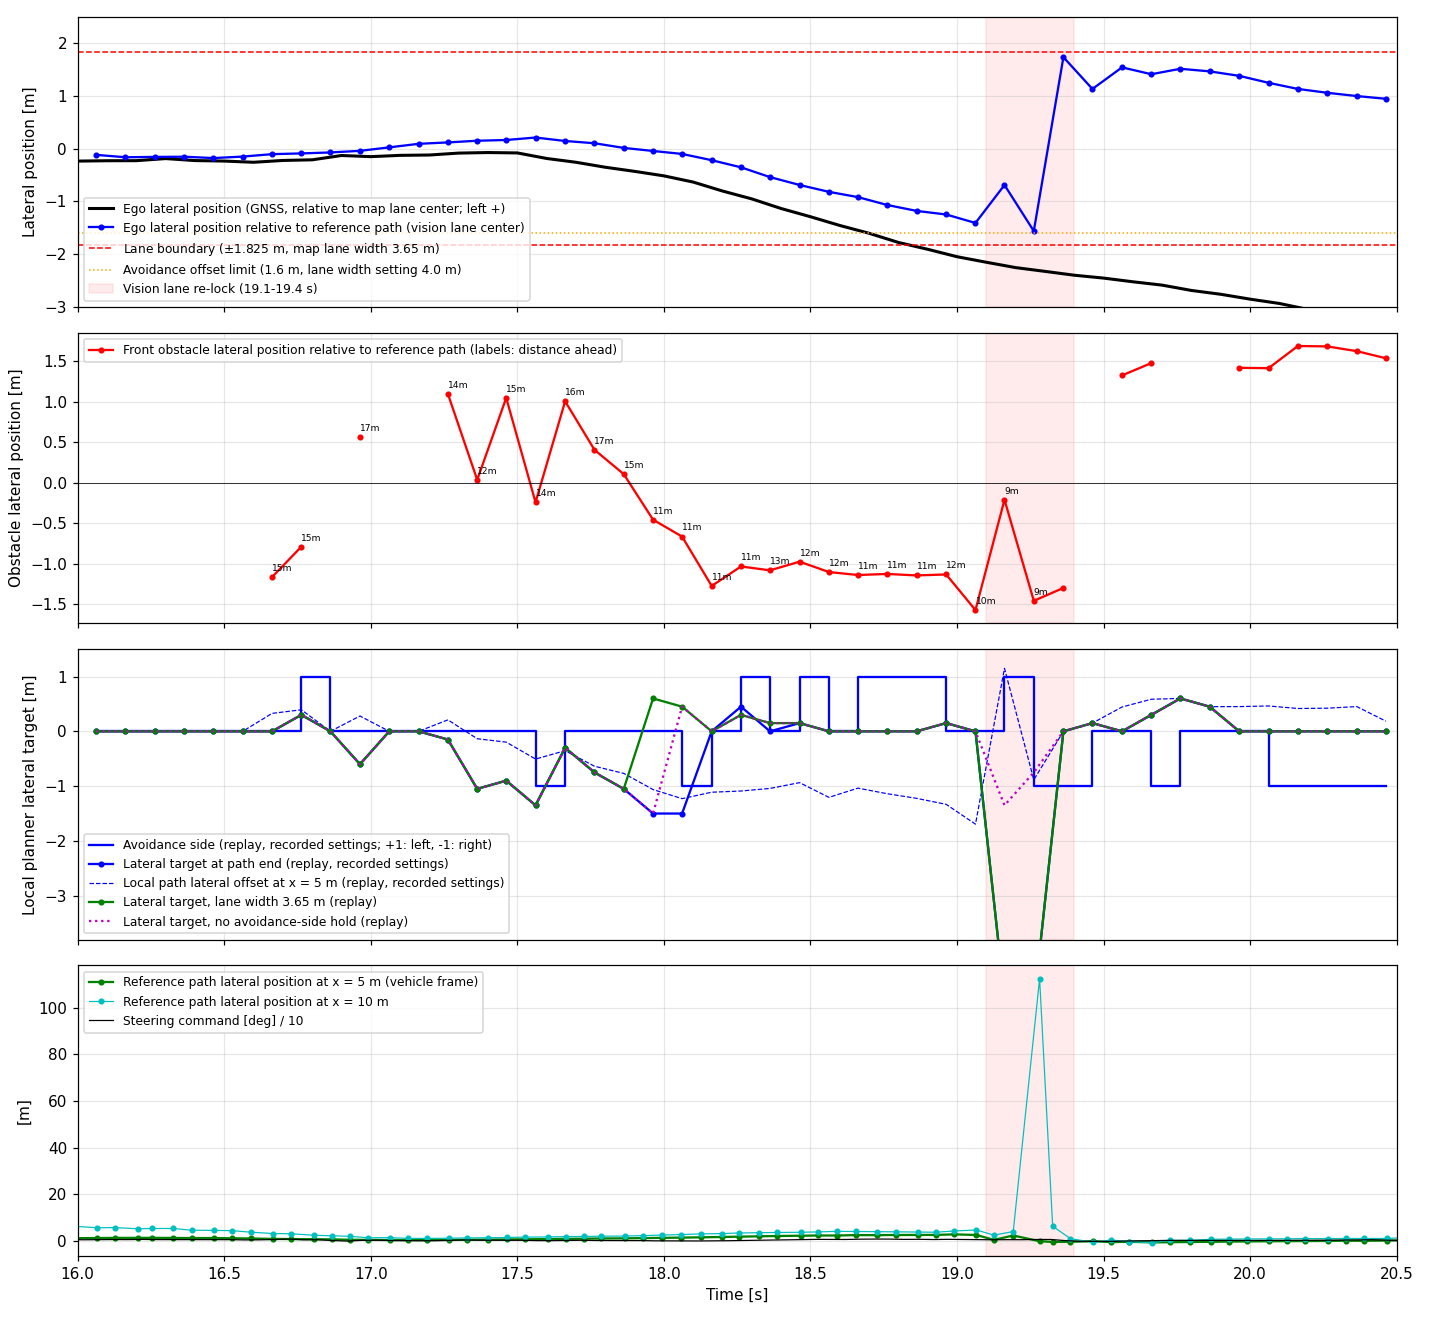
\includegraphics[width=0.95\textwidth]{images/run55_lanechange_timeseries.png}
  \caption{Lane change in R3 (red course at 5.5\,m/s). From top: lateral position of the ego vehicle (GNSS relative to the map lane center, and relative to the smoothed reference path, i.e., the vision lane center); lateral position of the front obstacle relative to the reference path; avoidance side and lateral target of the local planner (replay of the planner on the recorded inputs with the recorded settings, with a lane width setting of 3.65\,m, and without the avoidance-side hold); reference-path lateral position at 5 and 10\,m ahead and the steering command. The red band is the interval in which the vision lane estimate was re-locked onto the image lane (19.1--19.4\,s).}
  \label{fig:run55_ts}
\end{figure}

\begin{figure}[H]
  \centering
  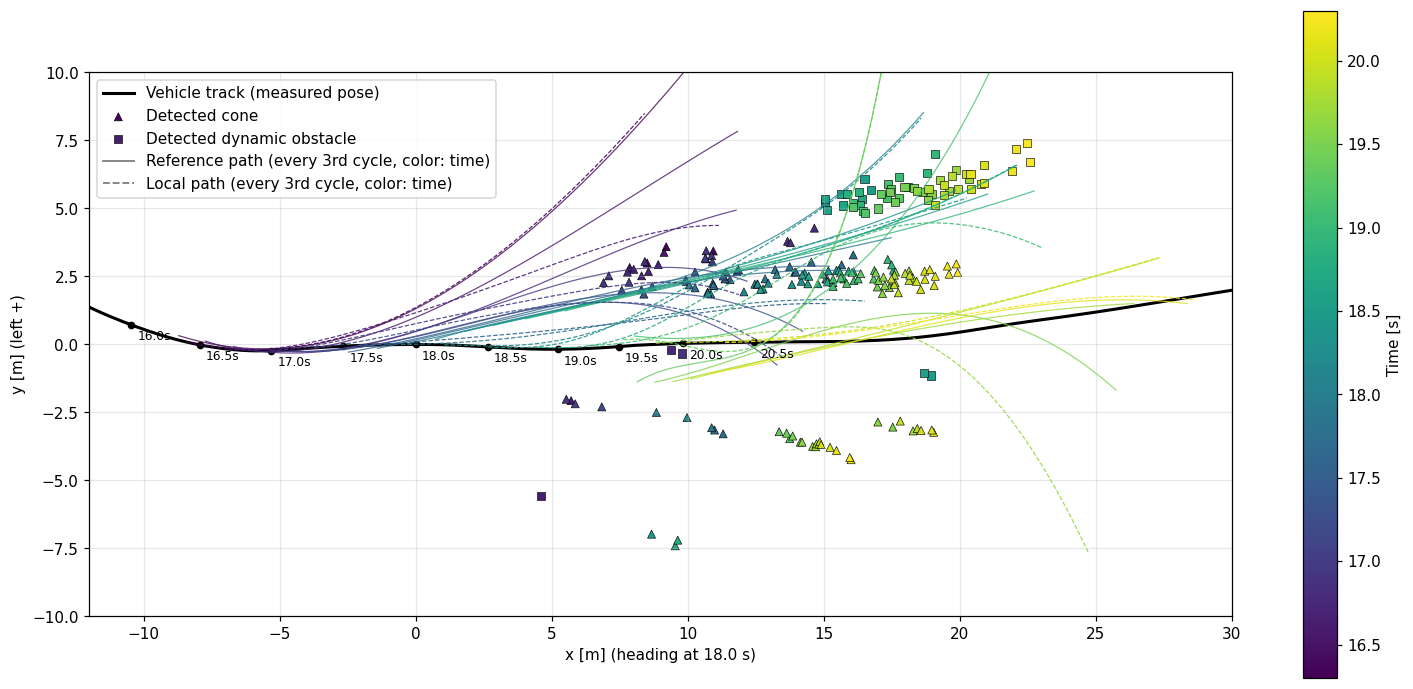
\includegraphics[width=0.9\textwidth]{images/run55_lanechange_topdown.png}
  \caption{Vehicle track (measured pose), reference paths (smoothed), local paths, detected cones, and detected dynamic obstacles in R3 from 16.3 to 20.3\,s (paths are drawn every third planning cycle).}
  \label{fig:run55_topdown}
\end{figure}

\begin{figure}[H]
  \centering
  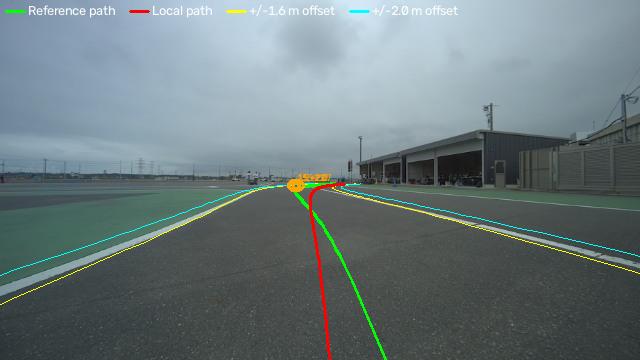
\includegraphics[width=0.8\textwidth]{images/run55_camera_overlay.png}
  \caption{Camera image and paths just before the lane change in R3. Green: reference path (smoothed), red: local path, yellow: $\pm 1.6$\,m offset (upper limit of the avoidance offset), cyan: $\pm 2.0$\,m offset (half of the lane width setting of 4.0\,m).}
  \label{fig:run55_cam}
\end{figure}

\subsection{経路生成}
10月27日の重み（10月24日版）による経路生成の出力の揺れは，前後1\,sの出力の中央値を基準とした前方5\,mでの横位置のずれが95パーセント点で約0.1\,mであり，4\,m/sと5\,m/sで差はなかった（10月12日の9月27日版の指標とは定義が異なるため直接は比べられない）．出力される経路の認識距離は中央値8.1\,mで，25\%のフレームで6\,m未満であった．交差点での急旋回中には経路が崩れる例があり，右折の指示が早い場合に手前の白線を誤検出する例があった（B7）．経路生成の誤差が主因と特定された失敗はこの1本であるが，前述のとおり多くの走行が短時間で打ち切られているため，高速での交差点通過において経路生成が十分に試されたとは言えない．

\section{ラップタイムの内訳}
\label{sec:decomp_result}
\ref{sec:decomposition}節の方法を，上限速度4\,m/s（B1は4.5\,m/s）の4本に適用した結果をTable~\ref{tab:decomp}に，1周あたりの内訳をFig.~\ref{fig:decomp}に示す．Table~\ref{tab:decomp}の1周あたりの値は，部分周を含む走行全体の合計を周長比の周回数で割った平均であり，Table~\ref{tab:laptimes}の周回ごとのラップタイムとは一致しない（例えば10月12日の71.9\,sは，Table~\ref{tab:laptimes}の2周の68.5\,sに，停止を含む3周目の部分周が加わった平均である）．Fig.~\ref{fig:decomp_ts}には，R2について実測速度と各速度列を走行距離に対して示す．軌跡の曲率は慣性航法装置のヨーレートと車輪速度から求め（$\sigma=1.0$\,mのガウス平滑．直線とカーブの判定には$\sigma=1.5$\,mで平滑した曲率を用いる），1周あたりの曲率の積分は6.27〜6.56\,radで$2\pi$と一致した．物理限界は上限速度6.0\,m/s，加速3.4\,m/s$^2$，減速3.6\,m/s$^2$，横加速度6.0\,m/s$^2$とし，速度計画の設定値は$a_{y,\max}=3.0$，$a_{x,\max}=3.0$\,m/s$^2$（10月12日は記録上の6.0\,m/s$^2$）とした．記録された速度計画の出力は，制御器と同じく0.3\,s先の点を参照した．残差$\Delta T_{\mathrm{res}}$は，\ref{sec:decomposition}節で述べたとおり構成上0であり（計算上も$10^{-4}$\,s未満），表には示さない．

\begin{table}[H]
  \centering
  \caption{Breakdown of the lap time for the runs at a 4\,m/s limit (totals over the analyzed laps, signed, in seconds).}
  \label{tab:decomp}
  \small
  \begin{tabular}{lrrrr}
    \toprule
    項目 & 10/12 赤 & R2 赤 & B1 青 & R8 赤 \\
    \midrule
    解析した周回 & 2.57 & 3.00 & 2.97 & 3.00 \\
    走行距離 [m] & 663.9 & 764.6 & 751.9 & 767.4 \\
    $T_{\mathrm{lap}}$ & 184.6 & 219.0 & 178.7 & 249.6 \\
    $T_{\mathrm{phys}}$ & 111.5 & 128.1 & 126.4 & 128.8 \\
    $\Delta T_{\mathrm{cap}}$ & $+55.0$ & $+63.4$ & $+41.4$ & $+63.7$ \\
    $\Delta T_{\mathrm{plan}}$ & $-0.2$ & $+0.1$ & $+0.7$ & $+0.1$ \\
    $\Delta T_{\mathrm{path}}$ & $-0.3$ & $-0.4$ & $+5.7$ & $+6.4$ \\
    $\Delta T_{\mathrm{track}}$ & $+6.0$ & $+5.2$ & $+4.5$ & $+16.5$ \\
    $\Delta T_{\mathrm{stop}}$ & $+12.6$ & $+22.5$ & 0 & $+34.2$ \\
    \midrule
    1周あたりの$T_{\mathrm{lap}}$ & 71.9 & 73.0 & 60.1 & 83.2 \\
    1周あたりの$T_{\mathrm{phys}}$ & 43.4 & 42.7 & 42.5 & 42.9 \\
    1周あたりの$\Delta T_{\mathrm{cap}}$ & 21.4 & 21.1 & 13.9 & 21.2 \\
    \bottomrule
  \end{tabular}
\end{table}

\begin{figure}[H]
  \centering
  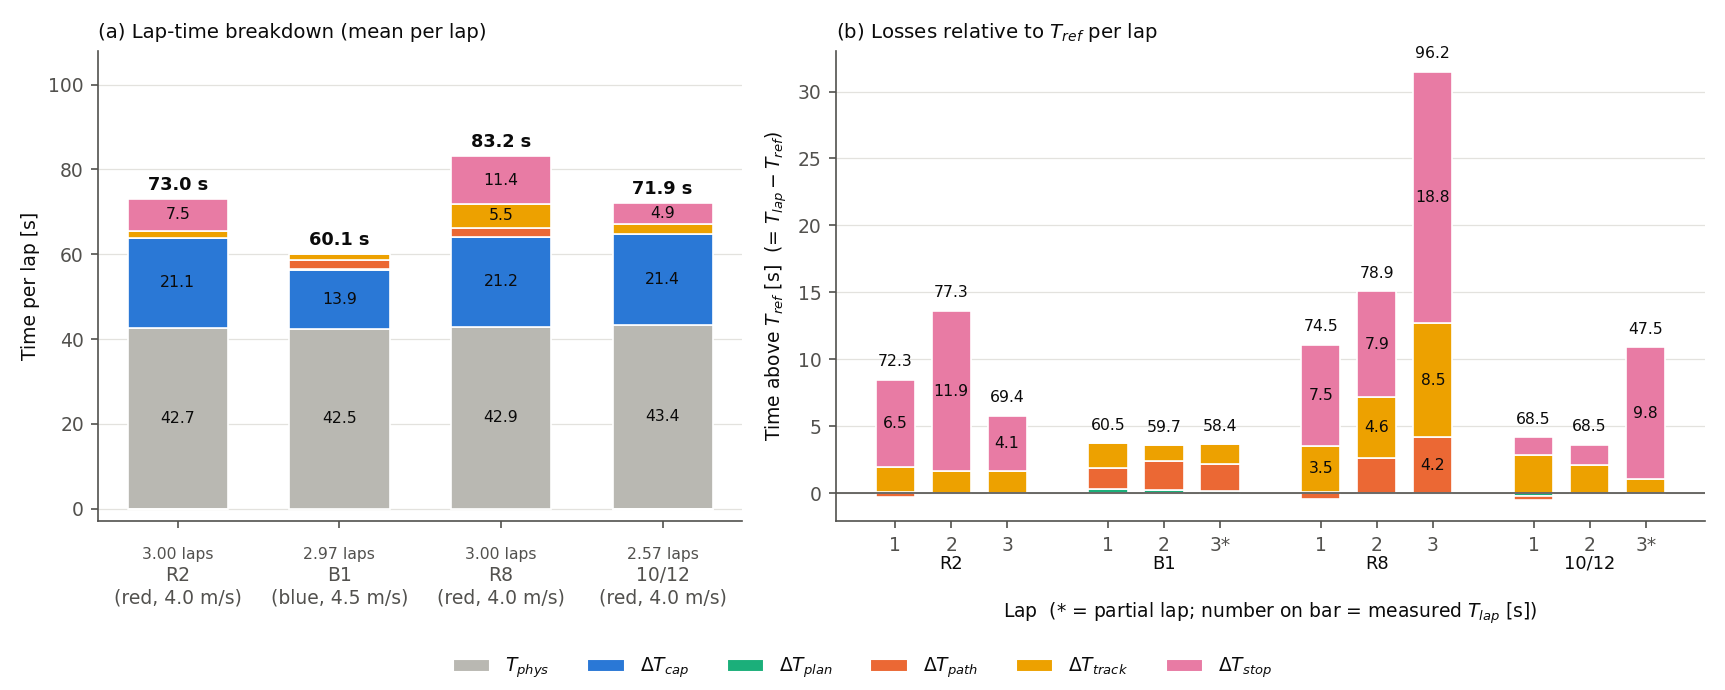
\includegraphics[width=0.98\textwidth]{images/decomp_4ms.png}
  \caption{Breakdown of the lap time per lap for the runs at a 4\,m/s limit: (a) mean per lap, (b) time above $T_{\mathrm{ref}}$ for each lap (numbers on bars are the measured lap times; * denotes a partial lap).}
  \label{fig:decomp}
\end{figure}

\begin{figure}[H]
  \centering
  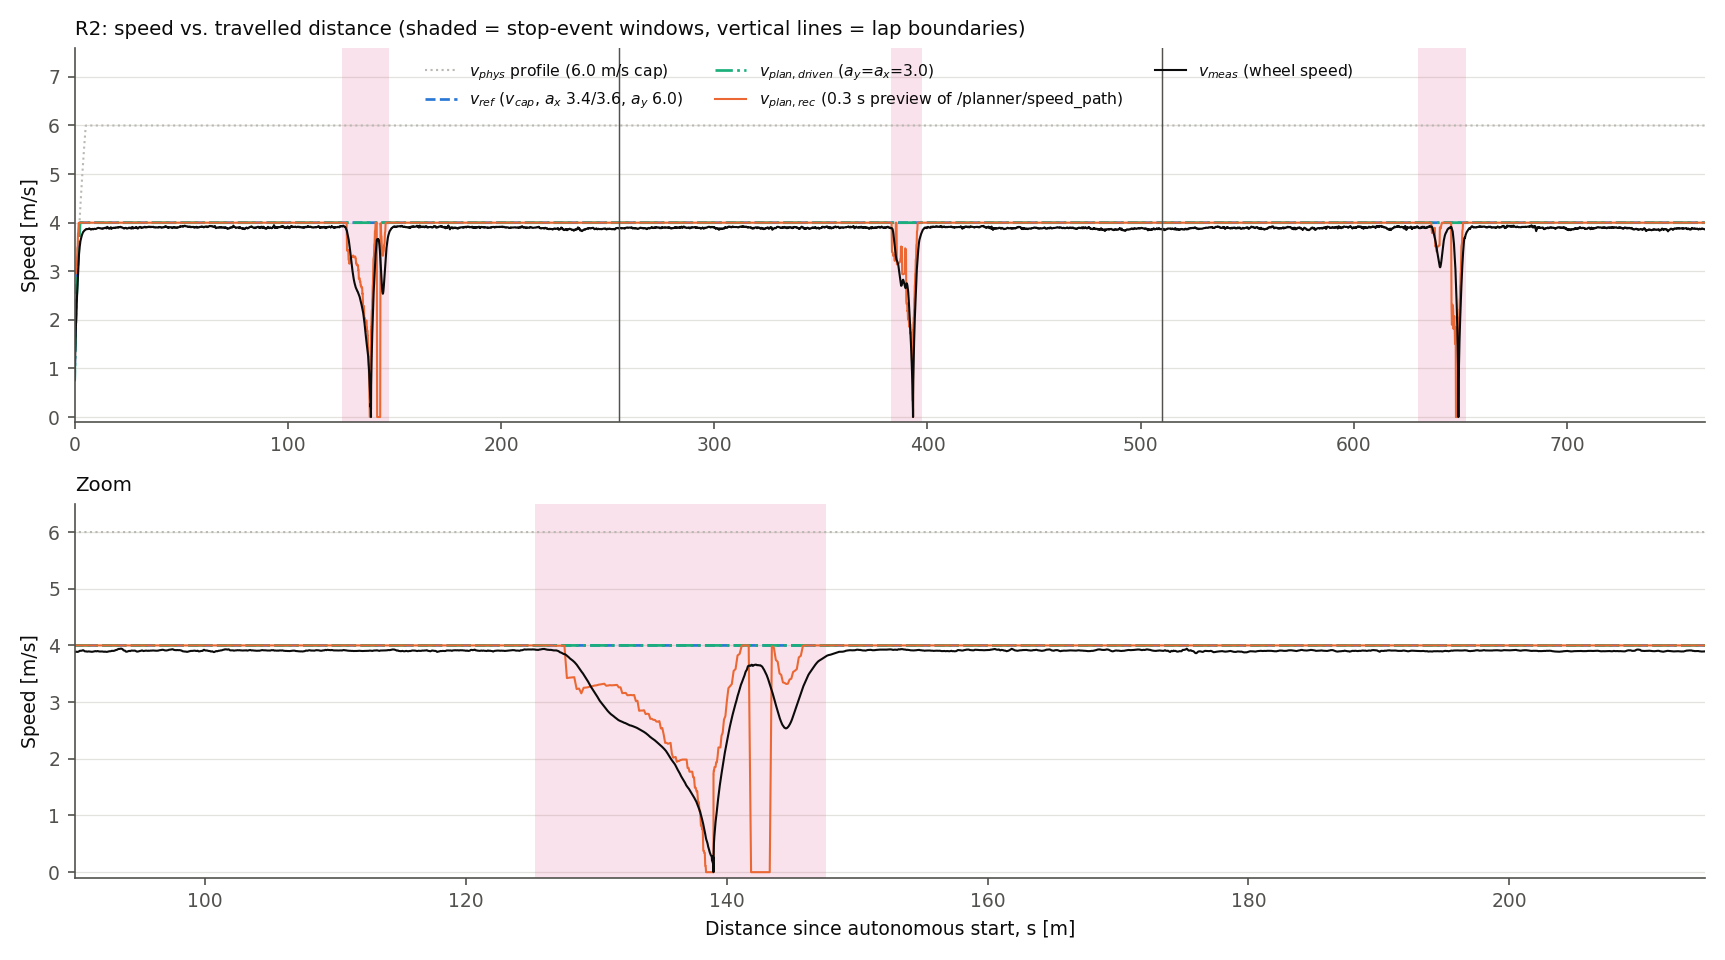
\includegraphics[width=0.98\textwidth]{images/decomp_timeseries.png}
  \caption{Measured velocity and the velocity profiles used in the decomposition versus travelled distance for R2 (red course, 4\,m/s limit). Shaded areas are the stop-event windows; the lower panel magnifies the second stop.}
  \label{fig:decomp_ts}
\end{figure}

赤コースの上限速度4\,m/sの3本では，1周あたり（解析した周回の平均）の$T_{\mathrm{lap}}$ 72〜83\,sのうち，物理限界だけで決まる$T_{\mathrm{phys}}$が約43\,s（52〜60\%），ソフトウェアの上限速度による$\Delta T_{\mathrm{cap}}$が約21\,s（26〜30\%），停止による$\Delta T_{\mathrm{stop}}$が1周あたり5〜11\,s（7〜14\%）を占める（10月12日の停止は消灯パネルの誤判定によるものであり，信号停止ではない）．速度計画の設定値と経路生成に由来する$\Delta T_{\mathrm{plan}}$と$\Delta T_{\mathrm{path}}$は，R2と10月12日では$\pm 0.4$\,s以内であるが，R8では$\Delta T_{\mathrm{path}}$が$+6.4$\,sである．上限速度$v_{\mathrm{cap}}$で走行軌跡を走った場合の横加速度$v_{\mathrm{cap}}^2|\kappa|$の最大値は赤コースで1.4〜1.8\,m/s$^2$（R2の実測の最大は1.3\,m/s$^2$）であり，速度計画の$a_{y,\max}=3.0$\,m/s$^2$は制約として働いていない．$T_{\mathrm{phys}}$の横加速度の上限を4.0〜6.0\,m/s$^2$の範囲で変えても，赤コースでは$T_{\mathrm{phys}}$は0.01\,s未満しか変わらない．実際，$v_{\mathrm{ref}}(s)$が$v_{\mathrm{cap}}$に等しい区間は4本とも走行距離の99.6〜99.7\%を占め，下回るのは発進直後の加速区間だけである．記録された計画速度$v_{\mathrm{rec}}$が$v_{\mathrm{cap}}$の95\%以上である区間も，停止窓を除くとR2と10月12日で99.8〜100\%であり，B1（76.8\%，交差点での上限4.0\,m/s）とR8（85.9\%，曲率の雑音による減速）でのみ減る．また，赤コースでは曲率による上限が走行可能な上限速度6.0\,m/sを下回る区間がないため，$T_{\mathrm{phys}}$は周長を上限速度で割った値にほぼ等しく，物理的な上限速度を5.5，6.0，6.5\,m/sとすると，$T_{\mathrm{phys}}$は1周あたり47.5，43.6，40.3\,s（R2）となり，$\Delta T_{\mathrm{cap}}$はその分だけ逆向きに変わる（$T_{\mathrm{ref}}$は不変）．ただし，これらの$T_{\mathrm{phys}}$と上の99.6〜99.7\%などの割合は，後述の車輪半径の較正（0.1265\,m）後の値であり，Table~\ref{tab:decomp}の$T_{\mathrm{phys}}$（R2で1周あたり42.7\,s，較正後の上限速度6.0\,m/sでは43.6\,s）とは異なる．すなわち，上限速度4\,m/sの段階で時間を決めているのは上限速度の設定であり，速度計画と経路生成の設定を変えても短縮の余地はほとんどない．

$\Delta T_{\mathrm{path}}$が大きかったのは，青コースのB1（$+5.7$\,s）と赤コースのR8（$+6.4$\,s）である．B1では，経路選択の指示が直進以外である3つの区間（計208.6\,m）で$+6.1$\,sを占め，それ以外の区間では$-0.4$\,sであった．このうち$+3.2$\,sは，分岐での速度抑制，すなわち指示が直進以外のあいだ速度計画の上限が4.5\,m/sから4.0\,m/sに下がったことによるもので，\ref{sec:decomposition}節で述べたとおり計算上は$\Delta T_{\mathrm{path}}$に入るが，速度計画の機能による時間差である．この分の走行距離118\,mは，指示が直進以外の3区間（208.6\,m）のうち，記録された計画速度が抑制値の4.0\,m/s（3.95〜4.05\,m/s）に一致していた区間の長さの合計であり，残りの区間（曲率と加減速で3.95\,m/s未満になった49.5\,mと，4.05\,m/sを超えた41.1\,m）では計画速度は抑制値に制限されていない．4.05\,m/sを超えた41.1\,mは，指示の切替直後の減速過渡や記録の時刻ずれを含む可能性があるが，確認していない．この分を$\Delta T_{\mathrm{plan}}$に移すと，B1の$\Delta T_{\mathrm{plan}}$は約$+3.9$\,s，$\Delta T_{\mathrm{path}}$は約$+2.5$\,sになる．残りの$+2.9$\,sは交差点の曲率と先読みによる減速である．B1では，上限速度で走った場合の横加速度$v_{\mathrm{cap}}^2|\kappa|$が最大4.2\,m/s$^2$で3.0\,m/s$^2$を超える区間が29.5\,mあったため，$\Delta T_{\mathrm{plan}}$も$+0.7$\,sとなった（実際の走行の横加速度の最大は3.4\,m/s$^2$，3.0\,m/s$^2$を超えた区間は3.4\,m）．R8では，3周目に経路の曲率の雑音による減速が繰り返され，$\Delta T_{\mathrm{path}}$と$\Delta T_{\mathrm{track}}$がともに大きい（3周目の$T_{\mathrm{lap}}$は96.2\,s）．ただしR8の$\Delta T_{\mathrm{track}}$の帰属は，後述の停止窓の定義にも依存する．$\Delta T_{\mathrm{path}}$が負になる区間は各走行の発進直後（$s<30$\,m）に集中しており，これは0.3\,s先の参照点が加速中に自車より高い速度を参照するためである．平滑化による曲率の過小評価が計画速度を高めた分は，データ上0.02\,s以下であった．10月12日の$\Delta T_{\mathrm{plan}}$が負（$-0.2$\,s）なのは，記録上の縦加速度の設定値6.0\,m/s$^2$が物理限界より大きいためである．

Table~\ref{tab:decomp_seg}に，直線とカーブに分けた集計を示す．停止による時間差はほぼすべて直線で生じ，B1とR8の$\Delta T_{\mathrm{path}}$はカーブに集中している．

\begin{table}[H]
  \centering
  \caption{Breakdown by straight and curved segments ($|\kappa|>0.04$\,1/m), in seconds.}
  \label{tab:decomp_seg}
  \scriptsize
  \begin{tabular}{lrrrrrr}
    \toprule
    走行 & path 直線 & path カーブ & track 直線 & track カーブ & stop 直線 & stop カーブ \\
    \midrule
    10/12 & $-0.3$ & $0.0$ & $+4.2$ & $+1.9$ & $+12.5$ & $+0.1$ \\
    R2 & $-0.4$ & $0.0$ & $+3.3$ & $+1.9$ & $+22.5$ & $0.0$ \\
    B1 & $+1.6$ & $+4.1$ & $+1.7$ & $+2.8$ & $0.0$ & $0.0$ \\
    R8 & $+0.3$ & $+6.1$ & $+5.9$ & $+10.7$ & $+33.4$ & $+0.9$ \\
    \bottomrule
  \end{tabular}
\end{table}

$\Delta T_{\mathrm{track}}$は1周あたり1.5〜2.3\,s（R2，B1，10月12日）および5.5\,s（R8）である．ただし，車輪速度は車輪半径0.124\,mで換算されており，GNSSの経路長との比較から実効半径は約0.1265\,m（約2\%大きい）と推定される．Fig.~\ref{fig:decomp_r1265}に，実効半径で距離と速度を換算し直した内訳を示す．$\Delta T_{\mathrm{track}}$はR2で$+1.7$\,s，B1で$+1.0$\,s，10月12日で$+3.0$\,s，R8で$+13.9$\,s（1周あたり0.6，0.3，1.2，4.6\,s）に減り，$T_{\mathrm{phys}}$と$T_{\mathrm{ref}}$は合計でそれぞれ2.2〜2.6\,s，3.3〜3.9\,s（1周あたり0.8〜0.9\,s，1.1〜1.3\,s）増える．赤コースの3本では，$T_{\mathrm{phys}}$の割合は53〜62\%，$\Delta T_{\mathrm{cap}}$は26〜30\%となり，$\Delta T_{\mathrm{path}}$と$\Delta T_{\mathrm{plan}}$は0.1\,s以内，$\Delta T_{\mathrm{stop}}$はR2と10月12日で0.4\,s以内しか変わらない（R8の$\Delta T_{\mathrm{stop}}$は合計で1.3\,s，1周あたり11.4\,sから11.0\,s減る）．したがって，R2，B1，10月12日の$\Delta T_{\mathrm{track}}$は較正で3.0〜3.5\,s減り（較正前の4.5〜6.0\,sの半分以上），その大部分は車輪半径の較正の不確かさの範囲内である．R8は2.6\,s減るがなお$+13.9$\,sと大きい．また，赤コースの3本では各項の大小の順序（$T_{\mathrm{phys}}$，$\Delta T_{\mathrm{cap}}$，$\Delta T_{\mathrm{stop}}$，$\Delta T_{\mathrm{track}}$，$\Delta T_{\mathrm{path}}$と$\Delta T_{\mathrm{plan}}$の順）は較正の前後で変わらない．B1は$\Delta T_{\mathrm{stop}}$が0で$\Delta T_{\mathrm{path}}$が$\Delta T_{\mathrm{track}}$より大きく（較正後$+5.9$\,s対$+1.0$\,s），この順序には当てはまらない．

\begin{figure}[H]
  \centering
  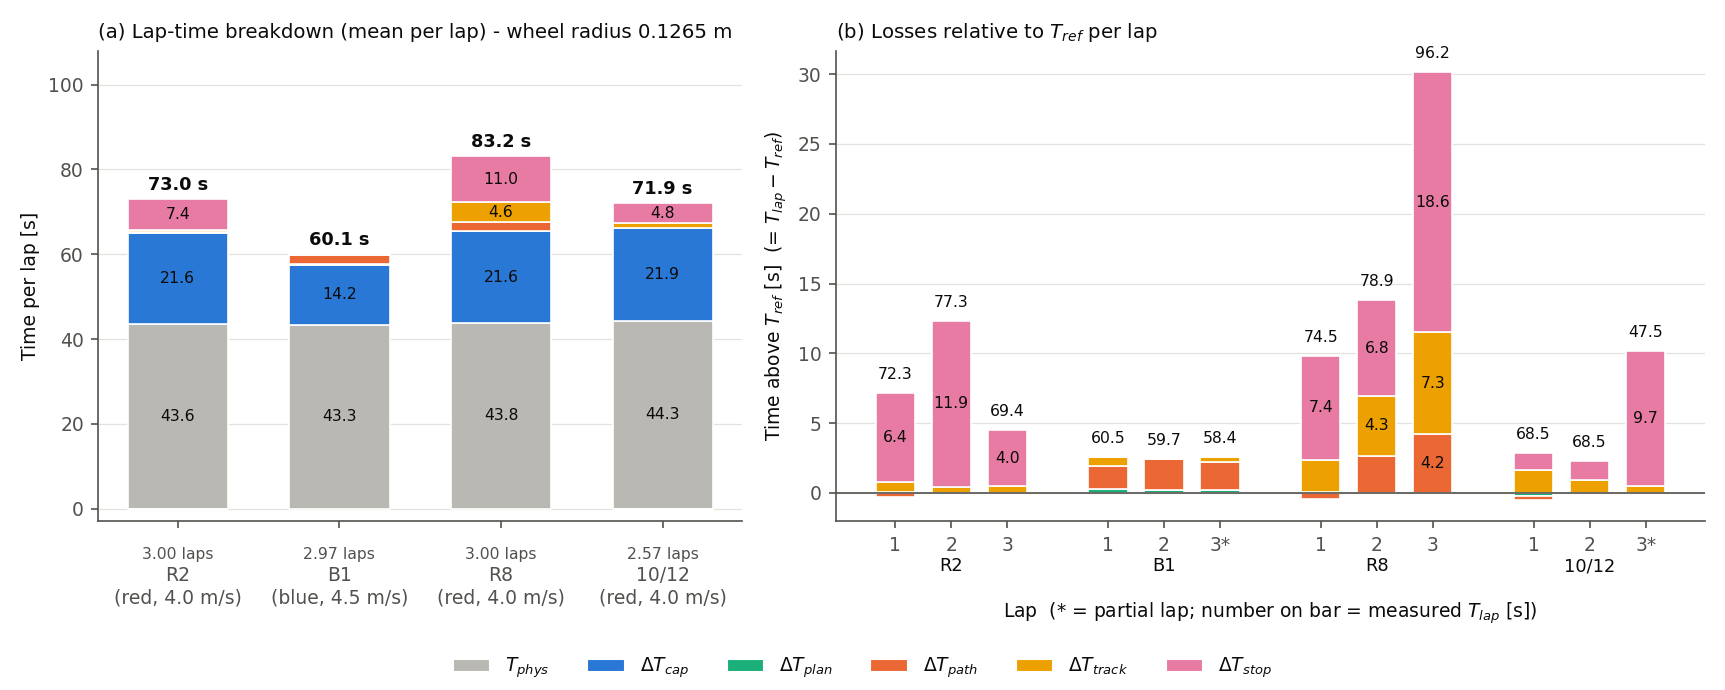
\includegraphics[width=0.98\textwidth]{images/decomp_4ms_r1265.png}
  \caption{Breakdown of the lap time per lap with the wheel speed and distance rescaled to the effective wheel radius of 0.1265\,m: (a) mean per lap, (b) time above $T_{\mathrm{ref}}$ for each lap.}
  \label{fig:decomp_r1265}
\end{figure}

$\Delta T_{\mathrm{stop}}$は停止1回あたり1.3〜18.8\,sと大きくばらつく．10月12日（消灯パネルの誤判定による停止，1.3〜9.8\,s）に対し，点灯パネルで停止した R2は4.1〜11.9\,s，R8は7.5〜18.8\,sであり，R8の3回目は停止後の再発進と再停止を含む．停止窓の終端の判定（計画速度の95\%への復帰）を90〜96\%の範囲で変えると，R2と10月12日では$\Delta T_{\mathrm{stop}}$の変化は0.2\,s以内である．R8では，2回目の窓の後の再加速中に速度の移動平均が一度しきい値を割るため，しきい値によって$\Delta T_{\mathrm{stop}}$が$\pm 1$\,s程度不連続に変わるが，$\Delta T_{\mathrm{track}}$と$\Delta T_{\mathrm{stop}}$の和は判定によらず一定である．巡航中の実測速度は計画値の約97.5\%（定常偏差と車輪半径の影響）であるため，98\%以上の判定では窓が閉じにくく，用いていない．

分解の定義に由来する不確かさは次のとおりである．記録された速度計画の参照点を0.3\,s先の点から最も近い点に変えると，R2では$\Delta T_{\mathrm{path}}$が$-0.4$\,sから$+3.8$\,sに，$\Delta T_{\mathrm{track}}$が$+5.2$\,sから$+1.1$\,sに変わり，両者の和は変わらない．曲率の平滑化の幅を0〜2\,mに変えると，B1の$\Delta T_{\mathrm{path}}$は$+5.1$〜$+6.1$\,s，$\Delta T_{\mathrm{plan}}$は$+1.4$〜$+0.3$\,sの範囲で変わり，和は約6.4\,sに保たれる．周回の切り方を基準線の通過から走行距離の等分に変えても，$T_{\mathrm{lap}}$の合計の差はR2とB1で0.07\,s以内，10月12日で0.29\,s以内，R8で最大0.96\,sであった．

\section{考察}
\label{sec:field_discussion}
赤コース（上限4.0\,m/s）のR2とR8は3周を完走し，青コース（上限4.5\,m/s）のB1は2.97周（3周目の97\%まで）を走行して手動で制動した．横偏差の95パーセント点は0.23〜0.79\,mであった．ラップタイムの内訳では，物理限界と上限速度の設定が赤コースで1周の77〜90\%（B1は94\%）を占め，速度計画の設定と経路生成に由来する時間差はR2と10月12日で$\pm 0.4$\,s以内，R8で$+6$\,s，青コースの交差点で$+6$\,sであった．ただし，上限速度4〜4.5\,m/sの4本は日付，コース，経路追従制御，平滑化の次数，経路生成の重みがいずれも異なる1本ずつの走行であり，走行間の差の原因や要素どうしの比較を実車の結果だけから述べることはできない．実車の結果が示すのは，これらの構成で上限速度4〜4.5\,m/sの2.97〜3周の走行（完走はR2とR8）が行えたという事実と，各走行の事例としての解析結果である．

5\,m/s以上では完走した走行はなく，主因の8本は自己位置推定の入力欠落と経路選択の初期化の不備であった．これらは速度計画や経路追従の設計とは独立したシステムの不具合であり，初期化の不備は速度と無関係に，入力欠落は走行の時刻（走行順）との関係が疑われるが，速度との交絡は解けていない．すなわち，5\,m/s以上では要素の設計の関与が特定できたのは2本（B7，R3）にとどまり（主因を特定できなかった3本は設計の関与を排除できない），8本では要素の設計による制約を観測する前に状態推定と初期化が正常に機能しなくなった．要素ごとの寄与を実車で評価するには，状態推定と初期化が正常に機能している上限速度の段階と条件（例えば慣性航法装置の出力の途絶がないこと）を前提として明示する必要がある．不具合を除いた条件で経路追従制御と車体の応答がどの速度まで成立するかは，5章の閉ループシミュレーションで評価する．
